\documentclass[11pt,a4paper]{report}
\usepackage[a4paper,margin=1in]{geometry}
\usepackage[T1]{fontenc}
\usepackage{times}
\usepackage{microtype}
\usepackage{booktabs,tabularx,array,longtable,multirow}
\usepackage{enumitem}
\usepackage{titlesec}
\usepackage{amsmath,amssymb}
\usepackage{float}
\usepackage{graphicx}
\usepackage{xcolor}
\usepackage{tikz}
\usetikzlibrary{positioning,arrows.meta,shapes.geometric}
\usepackage{algorithm}
\usepackage{algpseudocode}
\usepackage{caption}
\usepackage{fancyhdr}
\usepackage{url}
\usepackage[hidelinks]{hyperref}

\titleformat{\chapter}[hang]{\LARGE\bfseries}{\thechapter.}{0.6em}{}
\titlespacing*{\chapter}{0pt}{-10pt}{14pt}
\setlist{itemsep=2pt,topsep=4pt,leftmargin=1.4em}
\setlength{\parskip}{5pt}
\setlength{\parindent}{0pt}
\renewcommand{\arraystretch}{1.15}
\newcolumntype{Y}{>{\raggedright\arraybackslash}X}
\captionsetup{font=small,labelfont=bf}
\newcommand{\sys}[1]{\textsf{#1}}
\pagestyle{fancy}\fancyhf{}
\fancyhead[L]{\small CS683 NLP Project Report}\fancyhead[R]{\small Knowing When Not to Answer}
\fancyfoot[C]{\thepage}
\renewcommand{\headrulewidth}{0.4pt}

\emergencystretch=3em
\begin{document}

%================ TITLE PAGE ================
\begin{titlepage}
\centering
\vspace*{1.2cm}
{\large CS683 \,--\, Natural Language Processing\par}
\vspace{0.4cm}
{\large Course Project Report\par}
\vspace{2cm}
{\huge\bfseries Knowing When Not to Answer\par}
\vspace{0.4cm}
{\Large Abstention Drift in Multi-Turn\\Retrieval-Augmented Conversations\par}
\vspace{2.2cm}
{\large\bfseries Team Members\par}
\vspace{0.3cm}
{\large Member 1 \quad Member 2 \quad Member 3 \quad Member 4 \quad Member 5\par}
\vspace{2cm}
{\large Submitted to: \textit{Course Instructor, CS683}\par}
\vspace{0.3cm}
{\large M.Tech (Computer Science and Engineering)\par}
\vfill
{\large October 2026\par}
\end{titlepage}

%================ ABSTRACT ================
\pagenumbering{roman}
\chapter*{Abstract}
\addcontentsline{toc}{chapter}{Abstract}
Chat assistants built on retrieval-augmented generation (RAG) answer questions using documents they retrieve from a collection. When those documents do not contain the answer, the assistant should say ``I don't know'' (\emph{abstain}) instead of guessing. Most studies of this behaviour look at single questions, but real assistants hold long conversations.

This project asked two research questions. \textbf{RQ1:} does the assistant get worse at recognising unanswerable questions as a conversation goes on (\emph{abstention drift})? \textbf{RQ2:} can a small answerability checker, trained on unanswerable examples that we generate cheaply by removing the supporting documents, improve abstention without refusing more answerable questions?

We built a complete multi-turn RAG pipeline that runs on a 4\,GB laptop GPU. It uses the \textbf{Qwen2.5-3B-Instruct} large language model for query rewriting, answer generation and data filtering; \textbf{BM25} and the \textbf{BGE-small} embedding model for retrieval; the \textbf{BGE re-ranker} for re-ranking and as the answerability checker; and \textbf{DeBERTa-v3-base} for earlier checker versions. We evaluated six systems on the SemEval-2026 MTRAG-UN benchmark (429 turns, 97 unanswerable) and ran a controlled probe of 1{,}221 examples.

Results: (1) there is \textbf{no abstention drift}: recall on unanswerable questions stays flat across turns, and we can rule out declines larger than about one percentage point per turn; (2) 23\% of the cheaply generated ``unanswerable'' examples were actually still answerable and had to be filtered out; (3) no answerability checker improved the overall trade-off, as each one added more wrong refusals (8--13) than correct abstentions (3--8); (4) the main weakness of the pipeline is \textbf{over-refusal}: it refuses 18--28\% of questions that can be answered. Finally, we extended the pipeline with a \textbf{LangGraph agent} (built with LangChain) that searches again before refusing, asks clarifying questions and double-checks doubtful answers. Retrying before refusing cut wrong refusals from 18.4\% to 13.6\%, and adding a self-check calibrated on development data gave the best F1 of all systems (.511 vs .443 for the fixed pipeline). We then deployed the agent as a production web service (FastAPI, PostgreSQL, Qdrant, Celery, Guardrails AI, Langfuse, Prometheus and Grafana, with an automated quality gate in CI); running it end to end exposed and fixed a refusal-detection bug, which does not change any reported result, and two chunking problems for uploaded documents. Finally, we built a \textbf{NotebookLM-style web application} on the service (web, YouTube and text sources, source guides, a Studio with audio overviews, mind maps, flashcards and quizzes, sharing) with a choice of ten local open-weight models, whose refusal thresholds we calibrated per model: Qwen3-1.7B and Gemma-3-4B reached the best development F1 (.67 vs .62 for the research model). All code, predictions and scripts are available in the project repository.

\tableofcontents
\listoffigures
\listoftables

\clearpage
\pagenumbering{arabic}

%================ 1 INTRODUCTION ================
\chapter{Introduction}

\section{Background}
Large language models (LLMs) can answer questions fluently, but they sometimes produce confident answers that are not supported by any source (``hallucinations''). \emph{Retrieval-augmented generation} (RAG) reduces this problem: before answering, the system searches a document collection, retrieves the most relevant passages, and asks the LLM to answer using only those passages \cite{rag}. RAG is now the standard design for enterprise assistants, customer-support bots and document search tools.

RAG does not solve the problem completely. If the retrieved passages do not contain the answer, the model should reply ``I don't know''. In practice it often answers anyway, using partially related text or its own background knowledge. Declining to answer is called \emph{abstention}. Good abstention matters in the domains our data covers (finance, government services, technical documentation), where a wrong answer can mislead a user.

\section{Motivation}
Two observations motivated this project.
\begin{enumerate}
\item \textbf{Abstention is weak even in strong systems.} In the SemEval-2026 Task~8 (MTRAGEval) shared task on multi-turn RAG, one of the best systems reached 83.9\% answerability accuracy overall but detected only \textbf{21.8\%} of the unanswerable turns \cite{ails}.
\item \textbf{Abstention has mostly been studied on single questions} \cite{squad2,rgb,wen2025,feng}. Real users hold conversations: later questions are short, depend on earlier turns (``what about the second one?''), and the conversation history keeps growing. It is plausible that the assistant becomes \emph{worse} at knowing when not to answer as the conversation continues. We call this \emph{abstention drift}. No earlier work had measured it.
\end{enumerate}
A second practical problem is data: unanswerable turns are rare (6.5\% of the MTRAG training data), so training a detector needs a cheap way to create more examples.

\section{Research questions}
\begin{description}[leftmargin=1.2em,style=nextline]
\item[RQ1 -- Abstention drift] Does detection of unanswerable questions get worse at later turns of a conversation?
\item[RQ2 -- A cheap fix] Can a lightweight answerability checker, trained on unanswerable examples generated cheaply by \emph{evidence removal}, improve abstention without refusing more answerable questions (at most 5\% of answerable development turns refused)?
\end{description}

\section{Objectives}
\begin{enumerate}
\item Build a reproducible multi-turn RAG pipeline with query rewriting, hybrid retrieval, re-ranking and grounded answer generation that runs on a laptop GPU.
\item Measure abstention per turn position with proper statistics: confidence intervals, a controlled regression, and a controlled probe that removes the confound of question type.
\item Design and train an answerability checker using real and synthetic unanswerable examples, and compare it with simpler alternatives.
\item Analyse errors and report what limits abstention in practice.
\end{enumerate}

\section{Summary of outcomes}
\begin{itemize}
\item A working pipeline with six systems (\sys{S0}--\sys{S4} and \sys{S2-rr}) and a Gradio demo.
\item RQ1: no abstention drift on the test set or under the controlled probe.
\item RQ2: a negative result; synthetic data needed filtering (23\% noise), and no checker improved the trade-off.
\item A new finding: over-refusal of answerable questions is the main error (18--28\%).
\item An agentic extension (S5, LangGraph): retry before refusing lowers wrong refusals to 13.6\%; with a calibrated self-check it reaches the best F1 (.511); it asks clarifying questions on 37\% of underspecified turns.
\item A production service around the S5 agent: streamed answers, persistent conversations, document uploads, guardrails (0 of 1{,}349 real questions blocked, injection attempts blocked), tracing, metrics and a CI quality gate, tested end to end on the laptop.
\item A NotebookLM-style web application (sources, source guides, Studio, audio overviews, sharing) with a model menu of ten local models and refusal thresholds calibrated for each model.
\end{itemize}

\section{Organisation of this report}
Chapter~2 reviews related work. Chapter~3 describes the datasets and Chapter~4 the models used. Chapter~5 presents the system design and Chapter~6 the implementation. Chapter~7 describes the experiments and Chapter~8 the results. Chapter~9 presents the agentic extension built with LangChain and LangGraph, Chapter~10 the production service built around it, and Chapter~11 the NotebookLM-style application built on the service, including per-model refusal thresholds. Chapter~12 analyses errors, Chapter~13 lists the challenges we met and how we solved them, and Chapter~14 discusses the findings. Chapter~15 covers limitations and future work, and Chapter~16 concludes. The appendices list prompts, hyper-parameters and commands.

%================ 2 LITERATURE ================
\chapter{Literature Review}

\section{Multi-turn RAG benchmarks}
Conversational question-answering datasets such as CoQA \cite{coqa} and QuAC \cite{quac} include unanswerable questions, but each conversation is about one given passage, so there is no retrieval step. \textbf{MTRAG} \cite{mtrag} (TACL 2025) was the first benchmark of human-written multi-turn conversations over large document collections with answerability labels. \textbf{MTRAG-UN} \cite{mtragun} extends it with more unanswerable, underspecified and non-standalone questions and was used as the evaluation data for SemEval-2026 Task~8. Both benchmarks report performance on unanswerable questions as one overall number, and the SemEval system papers \cite{ails} focus on leaderboard scores; none analyses how abstention changes with turn position.

\section{Unanswerable questions and abstention}
SQuAD~2.0 \cite{squad2} added unanswerable questions to extractive reading comprehension. \emph{Selective prediction} lets a model decline when it is not confident \cite{selective,kamath}. For LLMs, researchers have studied whether models know what they know \cite{kadavath}, how several LLMs can collaborate to decide when to abstain \cite{feng}, and surveyed abstention methods \cite{wen2025}. In RAG, the RGB benchmark tests ``negative rejection'' when documents lack the answer \cite{rgb}, and Self-RAG trains the model to critique its retrieved passages \cite{selfrag}. All of these evaluate isolated questions.

\section{Query rewriting and retrieval}
Follow-up questions are hard to search with directly. Rewriting them into standalone questions is a standard step in conversational search \cite{canard}. For retrieval we combine the classic BM25 ranking function \cite{bm25} with dense embeddings from the BGE model family \cite{bge}, merge the two rankings with reciprocal rank fusion \cite{rrf}, and re-rank the result with a cross-encoder \cite{monobert}. Dense search uses the FAISS library \cite{faiss}.

\section{Generating unanswerable training data}
Unanswerable training examples are usually created by pairing questions with unrelated passages or by editing questions \cite{squad2}. Our \emph{evidence removal} keeps the real question and a realistic retrieval, and only removes the documents that contain the answer. To detect examples that remain answerable we use an LLM as a judge \cite{llmjudge}.

\section{Gap addressed by this project}
To our knowledge, no earlier work (i) measures abstention as a function of turn position while controlling for question type, or (ii) creates unanswerable training data for conversational RAG by removing evidence documents and measures how noisy that data is.

%================ 3 DATASETS ================
\chapter{Datasets}

\section{Task definition}
Each \emph{task} is one user turn in a conversation, together with the earlier turns (the history). The system must either answer from the retrieved passages or abstain with a fixed ``I don't know'' reply. Every task carries a human label: \textsc{answerable}, \textsc{partial}, \textsc{unanswerable}, \textsc{conversational} or \textsc{underspecified}. For our analysis:
\begin{itemize}
\item \textsc{unanswerable} $\rightarrow$ the system \emph{should abstain} ($y=1$);
\item \textsc{answerable} and \textsc{partial} $\rightarrow$ the system \emph{should answer} ($y=0$);
\item \textsc{conversational} and \textsc{underspecified} turns are excluded.
\end{itemize}

\section{MTRAG (training and development)}
MTRAG \cite{mtrag} (TACL 2025, IBM Research, Apache-2.0 licence) contains 110 human-written conversations with 7.7 turns on average, converted into 842 tasks: 709 answerable, 68 partial, 55 unanswerable and 10 conversational. Each task includes the reference (gold) passages, a reference answer and a human-written standalone rewrite of the question. We used MTRAG to train and tune the answerability checker, split 80/20 \emph{by conversation} (random seed 13) so that no conversation appears in both parts.

\section{MTRAG-UN (test)}
MTRAG-UN \cite{mtragun} (SemEval-2026 Task~8) contains 507 public tasks: 285 answerable, 47 partial, 97 unanswerable and 78 underspecified. It uses the same document collections. We used it only as the held-out test set. After removing underspecified turns, \textbf{429 tasks} remain: 97 unanswerable and 332 answerable (Table~\ref{tab:test}).

\begin{table}[H]
\centering\small
\begin{tabular}{@{}lrrr@{\hspace{2em}}lrr@{}}
\toprule
Domain & Unans. & Ans. & Total & Turn bucket & Unans. & Ans. \\
\midrule
ClapNQ & 22 & 83 & 105 & Turns 1--2 & 13 & 90 \\
Cloud & 36 & 86 & 122 & Turns 3--5 & 28 & 135 \\
FiQA & 12 & 58 & 70 & Turns 6+ & 56 & 107 \\
Govt & 27 & 105 & 132 & & & \\
\midrule
All & 97 & 332 & 429 & All & 97 & 332 \\
\bottomrule
\end{tabular}
\caption{MTRAG-UN test set used in this project, by domain and by turn bucket.}
\label{tab:test}
\end{table}

\section{Document collections}
The four passage-level collections shipped with MTRAG contain about 366K passages in total. Each passage is a chunk of up to 512 tokens (median 1{,}465 characters).
\begin{table}[H]
\centering\small
\begin{tabularx}{\textwidth}{@{}llY@{}}
\toprule
Collection & Source & Character \\
\midrule
ClapNQ & Wikipedia & General knowledge; the same topic often appears on many pages \\
Cloud & IBM Cloud documentation & Technical, specific pages \\
FiQA & Finance question-answer forums & Opinions and advice; many overlapping posts \\
Govt & U.S.\ government web pages & Services, regulations, public information \\
\bottomrule
\end{tabularx}
\caption{Document collections.}
\end{table}

\section{Self-created data: synthetic unanswerable examples}
From MTRAG we generated 507 synthetic unanswerable examples by evidence removal (Section~\ref{sec:er}) and kept 389 after filtering. Together with the real examples, the final checker data has 997 training and 224 development examples (Table~\ref{tab:checkerdata}).
\begin{table}[H]
\centering\small
\begin{tabular}{@{}lrrrr@{}}
\toprule
Split & Answerable (real) & Unanswerable (real) & Unanswerable (synthetic) & Total \\
\midrule
Train & 627 & 49 & 321 & 997 \\
Dev & 150 & 6 & 68 & 224 \\
\bottomrule
\end{tabular}
\caption{Answerability-checker data after filtering.}
\label{tab:checkerdata}
\end{table}

\section{The turn-position confound}
Unanswerable questions are not spread evenly over turns (Figure~\ref{fig:data}). In MTRAG-UN, 33.7\% of turns 6 and later are unanswerable, compared with 9.4\% of turns 1--2, because annotators usually asked unanswerable questions after a topic had been established. If we simply compare recall across turn positions, we mix the effect of conversation depth with the effect of \emph{which} questions appear late. Our evaluation controls for this (Sections~\ref{sec:logit} and~\ref{sec:probe}).
\begin{figure}[H]
\centering
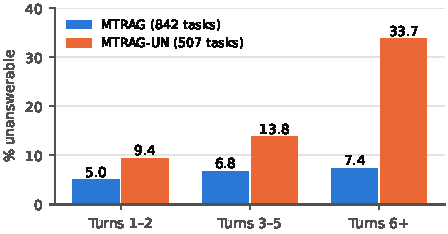
\includegraphics[width=0.62\textwidth]{fig_data.pdf}
\caption{Share of unanswerable tasks by turn position in MTRAG and MTRAG-UN (our analysis).}
\label{fig:data}
\end{figure}

%================ 4 MODELS ================
\chapter{Models Used}
This chapter lists every model used in the project, its role and how it was run. Table~\ref{tab:models} is the summary.

\begin{table}[H]
\centering\small
\begin{tabularx}{\textwidth}{@{}p{3.6cm}p{2.4cm}p{1.4cm}Y@{}}
\toprule
Model & Type & Size & Role in the project \\
\midrule
\textbf{Qwen2.5-3B-Instruct} \cite{qwen} (\texttt{qwen2.5:3b}, Q4\_K\_M) & Large language model (decoder) & 3.1B params & (1) query rewriting, (2) answer generation with prompt-only abstention, (3) LLM judge for filtering synthetic data; (4) in the S5 agent: retry rewriting, answer self-check and clarifying questions. Used in all systems. \\
\textbf{BM25} (\texttt{bm25s}) \cite{bm25} & Sparse lexical ranking & -- & First-stage retrieval in all systems. \\
\textbf{BAAI/bge-small-en-v1.5} \cite{bge} & Dense bi-encoder (embeddings) & 33M params, 384-dim & Dense retrieval in \sys{S2}--\sys{S4}. \\
\textbf{BAAI/bge-reranker-base} \cite{bge} & Cross-encoder (XLM-RoBERTa-base) & 278M params & (1) re-ranking in \sys{S2}--\sys{S4}; (2) untrained gate in \sys{S2-rr}; (3) initial weights of the final fine-tuned checkers in \sys{S3} and \sys{S4}. \\
\textbf{microsoft/deberta-v3-base} \cite{deberta} & Encoder (cross-encoder classifier) & 184M params & Earlier answerability checkers (5 training runs); replaced by the re-ranker-based checker. \\
\bottomrule
\end{tabularx}
\caption{Models used in the project. The S5 agent orchestrates these models with LangChain and LangGraph (Chapter~\ref{ch:agent}).}
\label{tab:models}
\end{table}

\section{Large language model: Qwen2.5-3B-Instruct}
\textbf{What it is.} Qwen2.5-3B-Instruct \cite{qwen} is an open instruction-tuned LLM from Alibaba's Qwen team with about 3.1 billion parameters and a 32K-token context window. It follows chat instructions well for its size and is released under a permissive licence.

\textbf{Why we chose it.} Our GPU (NVIDIA GTX~1650) has only 4\,GB of memory. A 7B model does not fit in 4-bit precision next to the retrieval models, while a 3B model quantised to 4 bits needs about 1.9\,GB. Our configuration also supports Qwen2.5-7B-Instruct for a larger GPU, but that setting was not run.

\textbf{How it was run.} We first loaded it with Hugging Face Transformers and bitsandbytes 4-bit quantisation, which took about 161 seconds per task on the laptop. We then switched to the \textbf{Ollama} runtime (llama.cpp) with the GGUF \texttt{Q4\_K\_M} quantisation of the same model (\texttt{ollama pull qwen2.5:3b}), which is several times faster. Decoding is greedy (temperature 0, fixed seed 13), so outputs are deterministic. The context window was set to 4{,}096 tokens.

\textbf{Its three roles.}
\begin{enumerate}
\item \textbf{Query rewriter:} turns a follow-up question into a standalone search query (max 64 new tokens).
\item \textbf{Answer generator:} writes the answer from the top-5 passages, or replies ``I'm sorry, but I don't have the answer to your question.'' when the passages are insufficient (max 128 new tokens). This is the \emph{prompt-only abstention} used by every system.
\item \textbf{LLM judge:} decides whether a synthetic ``unanswerable'' example is in fact still answerable (max 3 new tokens: ``yes''/``no'').
\item \textbf{Agent reasoning (S5):} writes alternative queries for retries, checks whether an answer is supported by the passages, and writes clarifying questions (Chapter~\ref{ch:agent}).
\end{enumerate}
The prompts are listed in Appendix~\ref{app:prompts}.

\section{Retrieval models}
\textbf{BM25} scores passages by overlapping words, weighted by how rare each word is. It needs no training and is strong on exact terms such as product names. We used the \texttt{bm25s} library with English stop words and took the top 100 passages.

\textbf{BGE-small-en-v1.5} \cite{bge} is a 33M-parameter embedding model that maps queries and passages to 384-dimensional vectors; similar meanings have similar vectors, so it finds paraphrases that BM25 misses. All 366K passages were encoded once (in fp16 on the GPU) and stored in FAISS flat inner-product indexes \cite{faiss}. Queries are prefixed with the instruction recommended by the model authors.

\section{Cross-encoder: BGE-reranker-base}
A \emph{cross-encoder} reads the query and a passage together and outputs one relevance score. This is more accurate than comparing two separate embeddings but slower, so it is applied only to the top 15 fused candidates. \texttt{bge-reranker-base} \cite{bge} is based on XLM-RoBERTa-base (278M parameters). We ran it in fp16 with a maximum of 256 tokens per pair. The same model plays three roles: re-ranker, training-free abstention gate (\sys{S2-rr}), and starting point of the fine-tuned checker (\sys{S3}, \sys{S4}).

\section{DeBERTa-v3-base (earlier checker)}
DeBERTa-v3-base \cite{deberta} is a 184M-parameter encoder that performs well on classification. Our first checker design fine-tuned it to classify (question, passages) pairs as answerable or unanswerable. It never matched the untrained re-ranker (Section~\ref{sec:checkerdev}), so it was replaced.

%================ 5 SYSTEM DESIGN ================
\chapter{System Design and Methodology}

\section{Architecture}
Figure~\ref{fig:arch} shows the pipeline. A question can be refused in two places: at the \emph{answerability gate} before generation, or by the \emph{generator} itself.

\begin{figure}[H]
\centering
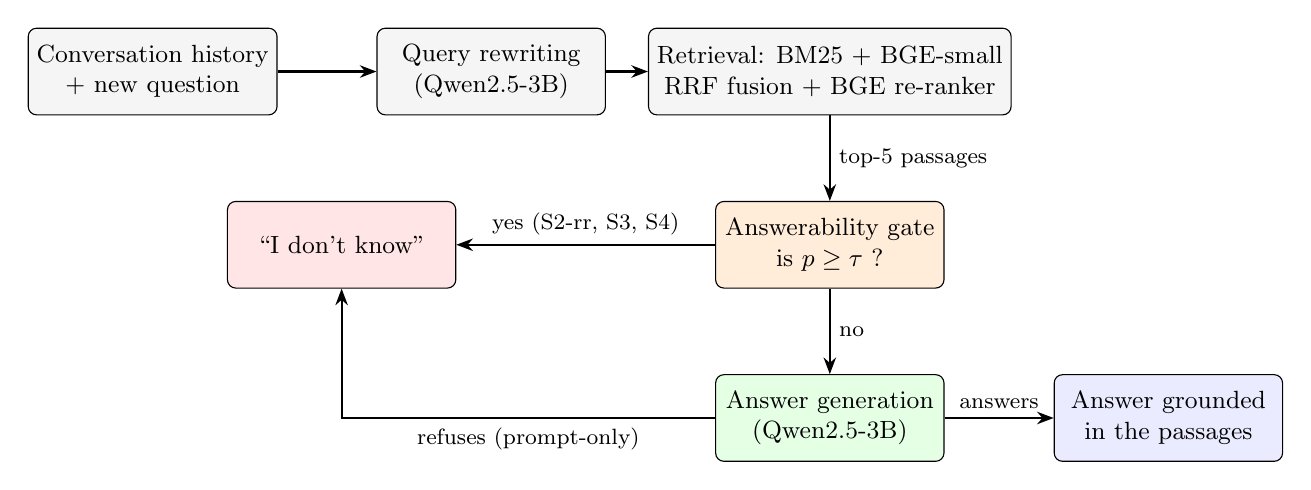
\begin{tikzpicture}[every node/.style={font=\small, align=center}, box/.style={draw, rounded corners=3pt, fill=gray!8, minimum height=1.1cm, minimum width=2.9cm, inner sep=3pt}, ar/.style={-{Stealth[length=6pt]}, thick}, lab/.style={font=\footnotesize, fill=white, inner sep=1pt}]
\node[box] (a) at (0,0) {Conversation history\\+ new question};
\node[box] (b) at (4.3,0) {Query rewriting\\(Qwen2.5-3B)};
\node[box] (c) at (8.6,0) {Retrieval: BM25 + BGE-small\\RRF fusion + BGE re-ranker};
\node[box, fill=orange!15] (d) at (8.6,-2.2) {Answerability gate\\is $p \ge \tau$ ?};
\node[box, fill=red!10] (f) at (2.4,-2.2) {``I don't know''};
\node[box, fill=green!10] (e) at (8.6,-4.4) {Answer generation\\(Qwen2.5-3B)};
\node[box, fill=blue!8] (g) at (12.9,-4.4) {Answer grounded\\in the passages};
\draw[ar] (a)--(b); \draw[ar] (b)--(c);
\draw[ar] (c)--node[lab,right=2pt]{top-5 passages}(d);
\draw[ar] (d)--node[lab,above=2pt]{yes (S2-rr, S3, S4)}(f);
\draw[ar] (d)--node[lab,right=2pt]{no}(e);
\draw[ar] (e) -| node[lab,pos=0.25,below=2pt]{refuses (prompt-only)}(f);
\draw[ar] (e)--node[lab,above=2pt]{answers}(g);
\end{tikzpicture}
\caption{Pipeline architecture.}
\label{fig:arch}
\end{figure}

\section{Stage 1: query rewriting}
The rewriter gives Qwen2.5-3B the last three exchanges of the history (each message cut to 400 characters) and the latest question, and asks for one standalone question. The first turn of a conversation is used unchanged. System \sys{S0} skips this step and searches with the raw last user turn.

\section{Stage 2: hybrid retrieval and re-ranking}
For each query, BM25 and the dense retriever each return 100 passages. Their rankings are merged by reciprocal rank fusion \cite{rrf}:
\[
\text{RRF}(d) = \sum_{r \in \{\text{BM25},\ \text{dense}\}} \frac{1}{60 + \text{rank}_r(d)} .
\]
The top 15 fused passages are re-scored by the BGE re-ranker, and the best $K=5$ are kept with their scores $s_1,\dots,s_5 \in [0,1]$.

\section{Stage 3: answer generation with prompt-only abstention}
The generator sees the five passages (each cut to 1{,}000 characters), the last three exchanges and the question. It is told to answer only from the passages and otherwise to give the fixed refusal. A reply counts as a refusal if its first 200 characters match one of six refusal patterns (for example ``I don't have the answer'' or ``the passages do not contain'').

\section{Stage 4: answerability gates}
A gate computes $p = P(\text{unanswerable})$ from the rewritten query and the five passages; if $p \ge \tau$ the system abstains without calling the generator.

\textbf{Untrained re-ranker gate (\sys{S2-rr}).} $p = 1 - \max_i s_i$: abstain when even the best passage is barely relevant.

\textbf{Fine-tuned checker (\sys{S3}, \sys{S4}).} The checker scores each (query, passage) pair separately and takes the minimum:
\[
p = \min_{i=1,\dots,5} P_\theta(\text{passage } i \text{ does not answer the query}), \qquad P_\theta = 1 - \sigma\big(z_\theta(q, P_i)\big),
\]
where $z_\theta$ is the relevance logit of the fine-tuned BGE re-ranker. A turn is judged answerable if \emph{any} passage answers it. Training pairs: every passage of an unanswerable example is a ``does not answer'' pair; the gold passages of an answerable example are ``answers'' pairs. \sys{S3} uses real labels only; \sys{S4} adds the filtered synthetic examples.

\textbf{Threshold.} On the development set we choose
\[
\tau^* = \arg\max_\tau \text{F1}_\text{abstain}(\tau) \quad\text{subject to}\quad \text{FA}(\tau) \le 5\%,
\]
where FA is the share of answerable development turns that the gate refuses. The chosen thresholds were 0.895 (\sys{S2-rr}), 0.543 (\sys{S3}) and 0.611 (\sys{S4}).

\section{Evidence removal: generating unanswerable examples}\label{sec:er}
For each answerable MTRAG turn we know which passages contain the answer. Algorithm~\ref{alg:er} removes \emph{all} passages from those source documents, retrieves again, and labels the new context unanswerable. This costs no annotation and produces realistic, closely related contexts. Answerable training examples are built the same way (retrieval with the gold passages inserted at random positions), so the checker cannot learn to spot gold passages by their position or style.

\begin{algorithm}[H]
\caption{Evidence removal for one answerable turn}
\label{alg:er}
\begin{algorithmic}[1]
\Require turn $x$ with rewritten query $q$, gold passages $G$, reference answer $a$
\State $\mathcal{D} \gets$ source documents of the passages in $G$
\State $R \gets$ \Call{Retrieve}{$q$}, excluding every passage of the documents in $\mathcal{D}$
\State $C \gets$ top-5 passages of $R$
\If{more than half of the content words of $a$ appear in $C$} \Return none \Comment{lexical filter}
\EndIf
\If{\Call{LLMJudge}{$x, a, C$} = ``yes''} \Return none \Comment{still answerable}
\EndIf
\State \Return $(q, C, \textsc{unanswerable})$
\end{algorithmic}
\end{algorithm}

\section{Systems compared}
\begin{table}[H]
\centering\small
\begin{tabularx}{\textwidth}{@{}lYl@{}}
\toprule
System & Components & Models involved \\
\midrule
\sys{S0} & Last user turn as query; BM25; prompt-only refusal & BM25, Qwen2.5-3B \\
\sys{S1} & \sys{S0} + LLM query rewriting & BM25, Qwen2.5-3B \\
\sys{S2} & \sys{S1} + dense retrieval, RRF fusion, re-ranking & + BGE-small, BGE-reranker \\
\sys{S2-rr} & \sys{S2} + gate on the untrained re-ranker score & same as \sys{S2} \\
\sys{S3} & \sys{S2} + fine-tuned checker, real labels only & + fine-tuned BGE-reranker \\
\sys{S4} & \sys{S2} + fine-tuned checker, real + synthetic labels (proposed) & + fine-tuned BGE-reranker \\
\bottomrule
\end{tabularx}
\caption{The six systems. Each adds one component to the previous one.}
\label{tab:systems}
\end{table}
Because generation is deterministic and the gate sits before the generator, \sys{S2-rr}, \sys{S3} and \sys{S4} give exactly the same outputs as \sys{S2} except where their gate fires. We therefore ran \sys{S2} once and derived the gated systems from its stored queries and passages.

%================ 6 IMPLEMENTATION ================
\chapter{Implementation}

\section{Hardware and software environment}
\begin{table}[H]
\centering\small
\begin{tabularx}{\textwidth}{@{}lY@{}}
\toprule
Item & Details \\
\midrule
Machine & Laptop, NVIDIA GeForce GTX~1650 (4\,GB VRAM, no bf16 support), 16\,GB RAM, 512\,GB SSD (OS) + 1\,TB HDD (project, data, models) \\
Operating system & Windows 11, Anaconda PowerShell Prompt, conda environment \texttt{abstain} \\
Language & Python 3.11 \\
Deep learning & PyTorch 2.14 with CUDA 12.6; Hugging Face Transformers 5; Accelerate; Datasets \\
Retrieval & \texttt{bm25s}, \texttt{sentence-transformers}, FAISS (CPU) \\
LLM serving & Ollama 0.34 (llama.cpp) for Qwen2.5-3B-Instruct GGUF; bitsandbytes for the Transformers backend \\
Agent framework & LangGraph 1.2, langchain-core 1.6, langchain-ollama 1.1 (\texttt{ChatOllama}) \\
Analysis & NumPy, pandas, scikit-learn (logistic regression), Matplotlib \\
Demo and tests & Gradio (interactive demo), pytest (26 research and 23 service tests), Ruff \\
Service (Ch.~\ref{ch:service}) & FastAPI, SQLAlchemy 2 + Alembic, PostgreSQL, Qdrant 1.19, Celery + Redis, Guardrails AI 0.11, Langfuse 3, OpenTelemetry, Prometheus, Grafana, Docker Compose, uv, GitHub Actions \\
\bottomrule
\end{tabularx}
\caption{Hardware and software.}
\end{table}

\section{Code organisation}
The code is a Python package with one script per step. Settings live in YAML configuration files: \path{configs/default.yaml} for a large GPU and \path{configs/laptop.yaml} for the 4\,GB laptop. In total the research package and scripts are about 2{,}450 lines of Python; the production service (Chapter~\ref{ch:service}) adds about 3{,}200.
\begin{table}[H]
\centering\small
\begin{tabularx}{\textwidth}{@{}lY@{}}
\toprule
Module / script & Purpose \\
\midrule
\texttt{src/abstain/data.py} & Load MTRAG / MTRAG-UN tasks and corpora, conversation split, turn buckets \\
\texttt{src/abstain/retrieval.py} & BM25 and dense indexes, RRF fusion, re-ranker, hybrid retriever \\
\texttt{src/abstain/llm.py} & LLM backends: Transformers (4-bit) and Ollama \\
\texttt{src/abstain/rewrite.py} & Query rewriting with the LLM \\
\texttt{src/abstain/generate.py} & Grounded answer generation prompt \\
\texttt{src/abstain/idk.py} & Refusal response and refusal detector \\
\texttt{src/abstain/checker.py} & Checker training and inference, re-ranker gate, threshold selection \\
\texttt{src/abstain/synth.py} & Evidence removal, lexical support filter, LLM judge \\
\texttt{src/abstain/pipeline.py} & End-to-end system with per-stage timing \\
\texttt{src/abstain/metrics.py} & Abstention metrics, drift slope with bootstrap, controlled regression \\
\texttt{scripts/*.py} & Build indexes, make and filter checker data, train checkers, run systems, apply gates, run probe, evaluate \\
\texttt{src/abstain/agent.py} & S5 LangGraph agent: LangChain wrappers, state graph, self-check, clarification \\
\texttt{app/app.py} & Gradio demo showing sources and a $P(\text{unanswerable})$ meter \\
\texttt{service/src/abstain\_api/} & Production service: API routers, agent runtime, retrieval (Qdrant/pgvector), uploads, guardrails, tracing, metrics, evaluation \\
\texttt{service/eval/}, \texttt{infra/}, \texttt{deploy/} & Quality-gate sample and baseline; Prometheus/Grafana configuration; Fly.io, Render, Kubernetes, Modal and RunPod deployment files \\
\bottomrule
\end{tabularx}
\caption{Main modules and scripts.}
\end{table}

\section{Implementation steps}
\begin{enumerate}
\item \textbf{Data setup:} download the MTRAG benchmark repository, compute dataset statistics.
\item \textbf{Indexing:} build BM25 and dense (BGE-small + FAISS) indexes for all four collections.
\item \textbf{Checker data:} rewrite queries with Qwen, retrieve, create answerable and evidence-removed examples.
\item \textbf{Filtering:} apply the LLM judge to every synthetic example (with a resumable cache).
\item \textbf{Checker training:} fine-tune the BGE re-ranker (\sys{S4}: real + synthetic; \sys{S3}: real only); fit the \sys{S2-rr} threshold.
\item \textbf{System runs:} run \sys{S0}, \sys{S1} and \sys{S2} on MTRAG-UN; derive \sys{S2-rr}, \sys{S3} and \sys{S4} from \sys{S2}.
\item \textbf{Probe and evaluation:} run the controlled probe and compute all metrics, confidence intervals and plots.
\end{enumerate}

\section{Checker training details}
\begin{itemize}
\item Initial weights: \texttt{BAAI/bge-reranker-base} (one relevance logit).
\item Loss: binary cross-entropy with class weights (the minority class is up-weighted by the class-frequency ratio).
\item Optimiser: AdamW, learning rate $10^{-5}$, 10\% warm-up, weight decay 0.01, 2 epochs, batch size 8 with 2 gradient-accumulation steps (effective 16), fp16, 256 tokens per pair.
\item Training pairs: 3{,}525 for \sys{S4} (1{,}849 ``does not answer''), 1{,}921 for \sys{S3} (245 ``does not answer''); 779 development pairs.
\item The checkpoint with the lowest development loss was kept. Training took 74 minutes (\sys{S4}) and 41 minutes (\sys{S3}).
\end{itemize}

\section{Efficiency measures}
Running an LLM pipeline on a 4\,GB GPU required several optimisations (details in Chapter~\ref{ch:challenges}):
\begin{itemize}
\item Ollama instead of bitsandbytes for the LLM: from about 161\,s to about 35\,s per task.
\item Shorter prompts (three history exchanges, 1{,}000-character passages): from 35.4\,s to 24.2\,s per task.
\item Deriving the gated systems from the \sys{S2} run: about 10 minutes per gate instead of about 3 hours per system.
\item Unloading the Ollama model from GPU memory before checker training.
\end{itemize}

%================ 7 EXPERIMENTS ================
\chapter{Experiments}

\section{List of experiments}
\begin{table}[H]
\centering\small
\begin{tabularx}{\textwidth}{@{}p{1.0cm}p{4.6cm}Yp{3.4cm}@{}}
\toprule
\# & Experiment & Purpose & Data \\
\midrule
1--6 & Systems \sys{S0}, \sys{S1}, \sys{S2}, \sys{S2-rr}, \sys{S3}, \sys{S4} & Abstention quality and drift (RQ1, RQ2) & MTRAG-UN, 429 turns \\
7 & Controlled probe: generator & Drift with question type fixed (RQ1) & MTRAG train+dev, 1{,}221 examples \\
8 & Controlled probe: checker & Drift of the \sys{S4} gate (RQ1) & MTRAG dev, 224 examples \\
9--13 & DeBERTa-v3 checkers (5 runs) & Checker development & MTRAG dev (256) \\
14--16 & BGE re-ranker: untrained, fine-tuned real only, fine-tuned real+synthetic & Checker development (RQ2) & MTRAG dev (224) \\
17 & LLM-judge filtering of synthetic data & Label-noise measurement & 507 synthetic examples \\
18 & Refusal-detector sensitivity analysis & Robustness of RQ1 conclusions & MTRAG-UN \\
19 & Dataset statistics by turn & Confound analysis & MTRAG, MTRAG-UN \\
20--23 & S5 agent: retry only, retry + self-check (always), self-check without retry, retry + selective self-check & Agentic extension & MTRAG-UN, 429 turns \\
24 & Self-check cut-off calibration & Choose min\_p on dev & MTRAG dev, 224 examples \\
25 & Clarification on underspecified turns & Agentic extension & MTRAG-UN, 78 turns \\
\bottomrule
\end{tabularx}
\caption{Experiments performed.}
\label{tab:exps}
\end{table}

\section{Evaluation metrics}
With $y_i=1$ for unanswerable turns and $\hat a_i=1$ when the system abstains (at the gate or in the generator):
\begin{itemize}
\item \textbf{Abstention recall} $= P(\hat a=1 \mid y=1)$: share of unanswerable turns correctly refused.
\item \textbf{Abstention precision} $= P(y=1 \mid \hat a=1)$: share of refusals that were justified.
\item \textbf{F1}: harmonic mean of abstention precision and recall.
\item \textbf{False-abstention rate (FA)} $= P(\hat a=1 \mid y=0)$: share of answerable turns wrongly refused (lower is better).
\item \textbf{AUROC} (for checkers): probability that a random unanswerable example gets a higher $p$ than a random answerable one (0.5 = chance, 1.0 = perfect).
\end{itemize}
All metrics are also reported per turn bucket: early (turns 1--2), mid (3--5), late (6+).

\section{Measuring abstention drift}
The \textbf{drift slope} $\beta$ is estimated from unanswerable turns with a linear-probability model
\[
P(\hat a_i = 1) = \alpha + \beta\, t_i ,
\]
where $t_i$ is the turn number. A negative $\beta$ means recall falls by $|\beta|$ per extra turn. Turns of one conversation are correlated, so the 95\% confidence interval comes from 1{,}000 bootstrap resamples of \emph{whole conversations}.

\section{Controlled regression}\label{sec:logit}
A logistic regression (scikit-learn) of $\hat a_i$ on $t_i$ with the domain (4 levels) and follow-up type (follow-up, clarification, none) as additional inputs separates the turn effect from question type. We report the \textbf{odds ratio per turn}: below 1 means abstention becomes less likely at later turns.

\section{Controlled probe}\label{sec:probe}
The probe holds question type fixed. Every answerable MTRAG turn gives two versions of the same question at the same turn position: one with the gold passages inserted (answerable) and one with the evidence removed (unanswerable). Only the passages differ. We fed these fixed inputs (a) to the \textbf{generator}, with the real conversation history, on train and development conversations (1{,}221 examples from 108 conversations; the generator is never trained, so using the training split is valid), and (b) to the \textbf{\sys{S4} checker}, on the development split only (224 examples from 22 conversations), because the checker was trained on the training split.

%================ 8 RESULTS ================
\chapter{Results}\label{ch:results}

\section{Main results}
\begin{table}[H]
\centering\small
\setlength{\tabcolsep}{2.5pt}
\begin{tabular}{@{}lccccccc@{}}
\toprule
& \multicolumn{4}{c}{Abstention (MTRAG-UN, $n=429$)} & \multicolumn{2}{c}{Drift per turn (95\% CI)} & Controlled \\
\cmidrule(lr){2-5}\cmidrule(lr){6-7}
System & F1 & Recall & Prec. & FA $\downarrow$ & Recall slope & FA slope & OR/turn \\
\midrule
\sys{S0} & .451 & \textbf{.567} & .374 & .277 & $-$.002 [$-$.048, +.046] & $-$.016 [$-$.037, +.004] & 0.99 \\
\sys{S1} & .453 & .526 & .398 & .232 & $-$.005 [$-$.051, +.041] & $-$.020 [$-$.040, $-$.000] & 0.97 \\
\sys{S2} & .443 & .464 & \textbf{.425} & \textbf{.184} & $-$.003 [$-$.046, +.043] & $-$.006 [$-$.022, +.012] & 1.00 \\
\sys{S2-rr} & \textbf{.473} & .546 & .417 & .223 & +.011 [$-$.031, +.057] & $-$.000 [$-$.018, +.018] & 1.06 \\
\sys{S3} & .457 & .515 & .410 & .217 & +.011 [$-$.030, +.055] & $-$.002 [$-$.019, +.018] & 1.06 \\
\sys{S4} & .449 & .495 & .410 & .208 & +.008 [$-$.034, +.051] & +.002 [$-$.015, +.020] & 1.04 \\
\midrule
Probe: generator & .489 & .423 & .578 & .176 & +.011 [$-$.010, +.029] & +.006 [$-$.005, +.016] & 1.08 \\
Probe: checker & .380 & .257 & .731 & .047 & +.000 [$-$.040, +.054] & +.006 [$-$.008, +.022] & 1.01 \\
\bottomrule
\end{tabular}
\caption{Main results. FA = share of answerable turns wrongly refused. Recall slope = change in abstention recall per extra turn. OR = odds ratio per turn from the controlled regression. Best system value per column in bold.}
\label{tab:main}
\end{table}

Table~\ref{tab:main} gives the main results. Abstention is hard for every system: F1 ranges from .443 to .473. The systems move along a trade-off rather than improving on it:
\begin{itemize}
\item \sys{S0} (weakest retrieval) refuses most often: highest recall (.567) but also the highest false-abstention rate (27.7\%).
\item Better retrieval (\sys{S1}, \sys{S2}) lowers false abstention to 18.4\% but also lowers recall to .464, because better passages also give the generator more material to answer unanswerable questions from.
\item The gates (\sys{S2-rr}, \sys{S3}, \sys{S4}) move \sys{S2} back towards more refusals.
\end{itemize}

\section{RQ1: abstention drift}
\begin{table}[H]
\centering\small
\begin{tabular}{@{}lcccccc@{}}
\toprule
& \multicolumn{2}{c}{Turns 1--2} & \multicolumn{2}{c}{Turns 3--5} & \multicolumn{2}{c}{Turns 6+} \\
\cmidrule(lr){2-3}\cmidrule(lr){4-5}\cmidrule(lr){6-7}
System & Recall & FA & Recall & FA & Recall & FA \\
\midrule
\sys{S0} & .538 & .289 & .536 & .319 & .589 & .215 \\
\sys{S1} & .462 & .267 & .500 & .252 & .554 & .178 \\
\sys{S2} & .538 & .156 & .393 & .222 & .482 & .159 \\
\sys{S2-rr} & .538 & .178 & .464 & .244 & .589 & .234 \\
\sys{S3} & .538 & .178 & .429 & .259 & .554 & .196 \\
\sys{S4} & .538 & .167 & .393 & .237 & .536 & .206 \\
\midrule
$n$ (unans. / ans.) & \multicolumn{2}{c}{13 / 90} & \multicolumn{2}{c}{28 / 135} & \multicolumn{2}{c}{56 / 107} \\
\midrule
Probe: generator & .404 & .154 & .401 & .178 & .460 & .192 \\
\quad $n$ & \multicolumn{2}{c}{104 / 208} & \multicolumn{2}{c}{177 / 298} & \multicolumn{2}{c}{163 / 271} \\
Probe: checker & .312 & .024 & .182 & .050 & .320 & .062 \\
\quad $n$ & \multicolumn{2}{c}{16 / 42} & \multicolumn{2}{c}{33 / 60} & \multicolumn{2}{c}{25 / 48} \\
\bottomrule
\end{tabular}
\caption{Abstention recall and false-abstention rate by turn bucket.}
\label{tab:bucket}
\end{table}

\begin{figure}[H]
\centering
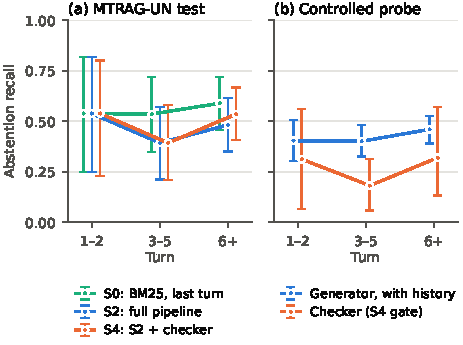
\includegraphics[width=0.75\textwidth]{fig_drift.pdf}
\caption{Abstention recall on unanswerable turns by turn position, with 95\% conversation-bootstrap confidence intervals. (a) MTRAG-UN test set; (b) controlled probe with question type held fixed.}
\label{fig:drift}
\end{figure}

\textbf{Finding: there is no abstention drift.}
\begin{itemize}
\item \textbf{Test set.} All six recall slopes lie between $-0.005$ and $+0.011$ per turn, and every 95\% confidence interval contains zero. With domain and follow-up type controlled, the odds ratios are 0.97--1.06, all close to 1. The per-bucket values (Table~\ref{tab:bucket}, Figure~\ref{fig:drift}a) show no downward trend. Because the early bucket has only 13 unanswerable turns, the test set alone can only exclude large drifts (about $\pm$0.045 per turn).
\item \textbf{Controlled probe.} With 444 unanswerable examples spread evenly across turns and question type fixed, the generator's recall is .404, .401 and .460. The slope is $+0.011$ [$-0.010$, $+0.029$] and the odds ratio 1.08. This rules out declines larger than about one percentage point per turn; if anything, the generator refuses slightly \emph{more} later in a conversation.
\item \textbf{Checker.} The checker never sees the conversation history, so it cannot drift by design. Its probe curve is flat (slope $+0.000$).
\end{itemize}

\textbf{Robustness check.} The refusal detector misses some hedged refusals (``I do not have specific information about \ldots''): 20 of the 429 \sys{S2} replies. Counting them as refusals raises \sys{S2}'s recall to .577 and FA to .211 (F1 .502), and \sys{S4}'s to .598 and .232 (F1 .500), but the drift slopes stay near zero: $+0.016$ [$-0.031$, $+0.065$] for \sys{S0}, $+0.002$ [$-0.041$, $+0.050$] for \sys{S2} and $+0.010$ [$-0.033$, $+0.058$] for \sys{S4}.

\section{RQ2: answerability gates}
\begin{figure}[H]
\centering
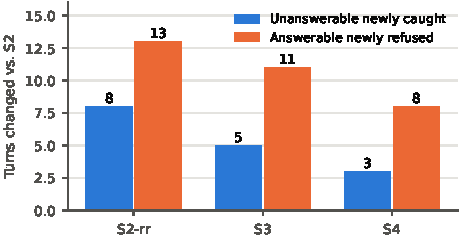
\includegraphics[width=0.62\textwidth]{fig_tradeoff.pdf}
\caption{Turns whose decision changes when each gate is added in front of \sys{S2}.}
\label{fig:tradeoff}
\end{figure}

\textbf{Finding: the gates do not pay off.} A gate can only add refusals to \sys{S2}. Compared with \sys{S2} (Figure~\ref{fig:tradeoff}):
\begin{itemize}
\item \sys{S2-rr} (untrained re-ranker) fires on 51 turns; it catches 8 more unanswerable turns but wrongly refuses 13 more answerable ones.
\item \sys{S3} (real labels only) catches 5 more and wrongly refuses 11 more.
\item \sys{S4} (real + synthetic labels) catches 3 more and wrongly refuses 8 more.
\end{itemize}
Every gate adds more wrong refusals than correct ones. F1 still rises slightly (to .473, .457 and .449) because recall on the rare unanswerable class carries much weight, but users would see more unjustified ``I don't know'' replies.

\textbf{Budget transfer.} Thresholds were chosen to refuse at most 5\% of answerable \emph{development} turns, yet test FA rose by 3.9 (\sys{S2-rr}), 3.3 (\sys{S3}) and 2.4 (\sys{S4}) percentage points: the development data (MTRAG, partly synthetic) differ from the test data (MTRAG-UN).

\textbf{Real vs.\ synthetic labels.} On the development set, fine-tuning on the 49 real unanswerable examples alone \emph{lowered} the re-ranker's AUROC from .741 to .660 (over-fitting to very few examples), while adding the filtered synthetic examples avoided this (.747). On the test set, however, \sys{S4} did not beat the untrained \sys{S2-rr}.

\section{Checker development}\label{sec:checkerdev}
\begin{table}[H]
\centering\small
\begin{tabular}{@{}clcc@{}}
\toprule
\# & Checker & \multicolumn{2}{c}{Dev AUROC (all / 6 real unans.)} \\
\cmidrule(lr){3-4}
& & Unfiltered dev (256) & Filtered dev (224) \\
\midrule
1 & DeBERTa-v3, passages concatenated, real + synthetic & .658 / .563 & -- \\
2 & DeBERTa-v3, passages concatenated, real only & .562 / .498 & -- \\
3 & DeBERTa-v3, one passage at a time, real + synthetic & .651 / .526 & -- \\
4 & DeBERTa-v3, one passage at a time, real only & .538 / .624 & -- \\
5 & BGE re-ranker, untrained (\sys{S2-rr}) & -- & .741 / .619 \\
6 & BGE re-ranker, fine-tuned, real only (\sys{S3}) & -- & .660 / .623 \\
7 & BGE re-ranker, fine-tuned, real + synthetic (\sys{S4}) & -- & \textbf{.747} / \textbf{.654} \\
\bottomrule
\end{tabular}
\caption{Checker development runs. ``6 real'' uses only the six real unanswerable development turns and is very noisy.}
\label{tab:checker}
\end{table}
We tried three designs (Table~\ref{tab:checker}):
\begin{enumerate}
\item \textbf{DeBERTa-v3, all passages concatenated.} The five passages were cut to 600 characters each and joined into one 384-token input. In 27 of 150 answerable development examples the gold passage was in position 3--5 and was partly or completely cut off. AUROC .66.
\item \textbf{DeBERTa-v3, one passage at a time.} Removed the truncation problem but did not help (.651).
\item \textbf{BGE re-ranker as the starting point.} The untrained re-ranker already reached .741; fine-tuning on real + synthetic data reached .747.
\end{enumerate}
Starting from a relevance model mattered more than the input design or the training data. Tuning the threshold on the six real unanswerable development turns alone (our first approach) was unreliable, since one example changes recall by 17 points; we therefore tuned on the full development set.

\section{Quality of the synthetic data}
\begin{table}[H]
\centering\small
\begin{tabular}{@{}lrrr@{}}
\toprule
Collection & Generated & Still answerable (dropped) & Share \\
\midrule
ClapNQ (Wikipedia) & 180 & 49 & 27\% \\
FiQA (finance) & 142 & 33 & 23\% \\
Govt (government) & 117 & 26 & 22\% \\
Cloud (IBM docs) & 68 & 10 & 15\% \\
\midrule
All & 507 & 118 & 23\% \\
\bottomrule
\end{tabular}
\caption{Synthetic examples judged still answerable by the Qwen2.5-3B LLM judge.}
\label{tab:synth}
\end{table}
Reading the synthetic examples showed many that could still be answered. For instance, ``Who funds the Europa Clipper mission?'' still retrieved several pages titled ``NASA's Europa Clipper'', and ``What intern programs does NASA have?'' retrieved three JPL ``STEM Internships'' pages. Removing the source \emph{document} does not remove the \emph{fact} when the collection repeats it on other pages. The LLM judge dropped 118 of 507 examples (23\%, Table~\ref{tab:synth}), most often in ClapNQ, where Wikipedia covers popular topics on many pages, and least in Cloud, whose documentation pages are more specific. After filtering, 321 training and 68 development synthetic examples remained (from 407 and 100).

The lexical filter alone was not enough. Reference answers of real answerable turns share most of their words with their passages (median overlap .87--.90) and synthetic examples far fewer (.30--.32), yet many low-overlap synthetic examples were still answerable through paraphrase.

\section{Over-refusal}
\begin{figure}[H]
\centering
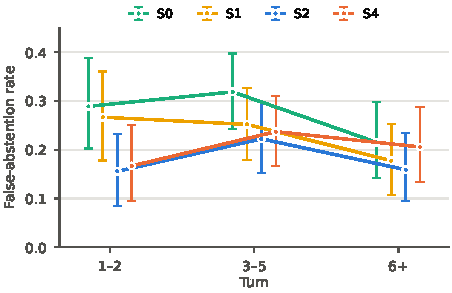
\includegraphics[width=0.62\textwidth]{fig_fa.pdf}
\caption{False-abstention rate (answerable turns refused) by turn position, with 95\% confidence intervals.}
\label{fig:fa}
\end{figure}
\textbf{Finding: over-refusal is the largest error.} Even the best retrieval (\sys{S2}) refuses 18.4\% of answerable turns (61 of 332), while it misses 52 of the 97 unanswerable turns. Without query rewriting, wrong refusals are highest early and mid-conversation (\sys{S0}: .289, .319, .215). With rewriting (\sys{S1}) they fall steadily from .267 to .178 (slope $-0.020$ per turn, the only confidence interval that excludes zero), possibly because opening questions are short and generic and retrieve less specific passages (Figure~\ref{fig:fa}).

\section{Results by domain}
\begin{table}[H]
\centering\small
\begin{tabular}{@{}lcccc@{}}
\toprule
& \multicolumn{2}{c}{\sys{S2}} & \multicolumn{2}{c}{\sys{S4}} \\
\cmidrule(lr){2-3}\cmidrule(lr){4-5}
Domain (unans. / ans.) & Recall & FA & Recall & FA \\
\midrule
ClapNQ (22 / 83) & .41 & .23 & .41 & .24 \\
Cloud (36 / 86) & .44 & .09 & .50 & .12 \\
FiQA (12 / 58) & .58 & .14 & .58 & .17 \\
Govt (27 / 105) & .48 & .25 & .52 & .28 \\
\bottomrule
\end{tabular}
\caption{Abstention by domain on MTRAG-UN.}
\label{tab:domain}
\end{table}
Over-refusal is concentrated in ClapNQ and Govt (23--28\% FA), whose varied web and Wikipedia pages often contain the answer in a form the 3B generator does not recognise. Cloud documentation is refused least (9\%). The \sys{S4} gate helps most in Cloud (+6 points recall for +3 points FA) and not at all in ClapNQ.

%================ AGENT ================
\chapter{Agentic Extension: LangGraph Self-Correcting Agent (S5)}\label{ch:agent}

\section{Motivation}
The fixed pipeline (\sys{S2}--\sys{S4}) rewrites the question once, retrieves once, and then either answers or refuses. Chapter~\ref{ch:results} (and the error analysis in Chapter~\ref{ch:errors}) showed where this fails: the largest error is \emph{over-refusal} (18.4\% of answerable turns for \sys{S2}), and several refusals start with a bad query rewrite. A human assistant who cannot find an answer would search again with different words, ask what the user means, or double-check a doubtful answer. We added these behaviours as a small \emph{agent} built with LangChain's LangGraph framework.

\section{Design}
The agent is a LangGraph \texttt{StateGraph}: each step is a node, the state (question, history, queries tried, passages, gate score, answer, decision, trace) flows between nodes, and conditional edges decide what happens next (Figure~\ref{fig:agent}).

\begin{figure}[H]
\centering
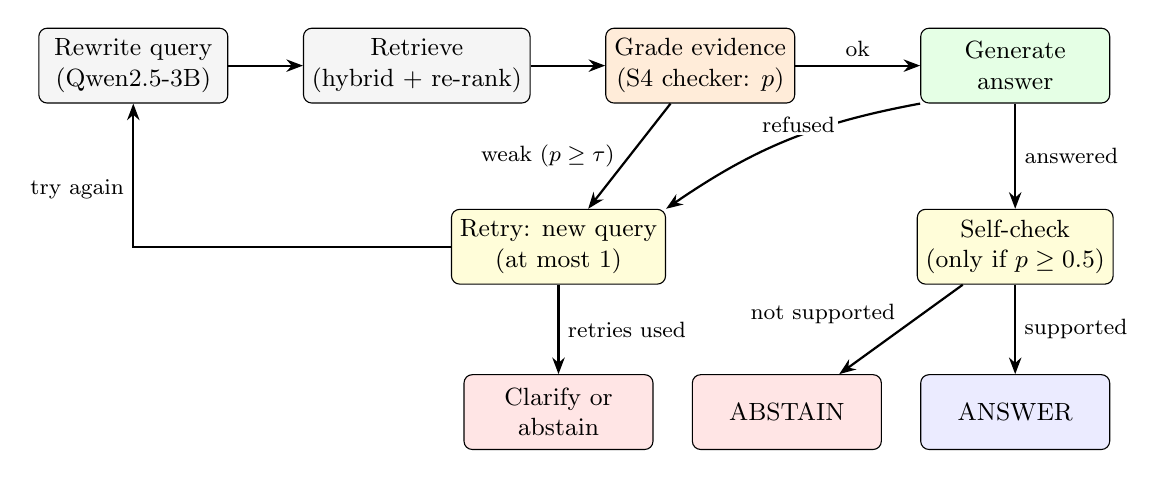
\begin{tikzpicture}[every node/.style={font=\small, align=center}, box/.style={draw, rounded corners=3pt, fill=gray!8, minimum height=0.95cm, minimum width=2.4cm, inner sep=3pt}, ar/.style={-{Stealth[length=6pt]}, thick}, lab/.style={font=\footnotesize, fill=white, inner sep=1pt}]
\node[box] (rw) at (0,0) {Rewrite query\\(Qwen2.5-3B)};
\node[box] (rt) at (3.6,0) {Retrieve\\(hybrid + re-rank)};
\node[box, fill=orange!15] (gr) at (7.2,0) {Grade evidence\\(S4 checker: $p$)};
\node[box, fill=green!10] (ge) at (11.2,0) {Generate\\answer};
\node[box, fill=yellow!15] (sc) at (11.2,-2.3) {Self-check\\(only if $p \ge 0.5$)};
\node[box, fill=blue!8] (ans) at (11.2,-4.4) {ANSWER};
\node[box, fill=yellow!15] (re) at (5.4,-2.3) {Retry: new query\\(at most 1)};
\node[box, fill=red!10] (ca) at (5.4,-4.4) {Clarify or\\abstain};
\node[box, fill=red!10] (ab) at (8.3,-4.4) {ABSTAIN};
\draw[ar] (rw)--(rt); \draw[ar] (rt)--(gr);
\draw[ar] (gr)--node[lab,above=2pt]{ok}(ge);
\draw[ar] (gr)--node[lab,left=4pt]{weak ($p \ge \tau$)}(re);
\draw[ar] (ge)--node[lab,right=2pt]{answered}(sc);
\draw[ar] (ge.south west) to[bend right=12] node[lab,pos=0.45,above]{refused}(re.north east);
\draw[ar] (sc)--node[lab,right=2pt]{supported}(ans);
\draw[ar] (sc)--node[lab,above left=1pt]{not supported}(ab);
\draw[ar] (re.west) -| node[lab,pos=0.7,left=2pt]{try again}(rw.south);
\draw[ar] (re)--node[lab,right=2pt]{retries used}(ca);
\end{tikzpicture}
\caption{The S5 agent as a LangGraph state graph.}
\label{fig:agent}
\end{figure}

\begin{enumerate}
\item \textbf{First attempt.} Rewrite, retrieve and grade exactly as in \sys{S2}/\sys{S4}; the S4 checker gives the gate score $p$ ($\tau = 0.611$).
\item \textbf{Retry before refusing.} If the evidence is weak ($p \ge \tau$) or the generator refuses, Qwen writes a \emph{different} query, told to expand abbreviations, keep the user's own key words and not carry over an earlier topic, and is shown the queries already tried. The agent retrieves and grades again (one retry).
\item \textbf{Clarify or abstain.} If the retry also fails, Qwen judges whether the question is ambiguous. If yes, the agent asks one short clarifying question; otherwise it abstains. In the binary metrics a clarifying question counts as not answering.
\item \textbf{Selective self-check.} After an answer, Qwen judges whether the answer's main claim is supported by the passages; if not, the agent abstains. The check runs only when the gate already doubts the evidence ($p \ge$ min\_p, Section~\ref{sec:selective}).
\end{enumerate}

We deliberately used \textbf{fixed, rule-based routing} rather than a free ``tool-calling'' (ReAct) agent: a 3B model follows explicit steps reliably but chooses tools poorly, and fixed routing keeps the agent easy to evaluate and explain.

\section{Implementation with LangChain and LangGraph}
\begin{itemize}
\item \textbf{LLM:} Qwen2.5-3B-Instruct through LangChain's \texttt{ChatOllama} (\texttt{langchain-ollama}), temperature 0, seed 13, with automatic retries on server errors. The existing rewriting and generation prompts are reused unchanged.
\item \textbf{Retriever:} a LangChain \texttt{BaseRetriever} subclass wrapping our hybrid BM25 + BGE-small + re-ranker retriever, returning LangChain \texttt{Document} objects.
\item \textbf{Graph:} a LangGraph \texttt{StateGraph} with seven nodes (\texttt{rewrite}, \texttt{retrieve}, \texttt{grade}, \texttt{generate}, \texttt{self\_check}, \texttt{retry}, \texttt{clarify\_or\_abstain}) and three conditional edges. Code: \texttt{src/abstain/agent.py} (about 300 lines); versions LangGraph 1.2, langchain-core 1.6, langchain-ollama 1.1.
\item \textbf{Trace:} every prediction stores the queries tried, the gate scores, each decision and the final outcome, so every agent decision can be inspected.
\item \textbf{Efficient evaluation:} the agent's first attempt is identical to \sys{S2}, so \texttt{run\_agent.py} reuses the stored \sys{S2} queries, passages and answers and the \sys{S4} gate scores; only the new steps call the LLM. The run is resumable.
\item \textbf{Tests:} seven unit tests drive the graph with a scripted fake LLM and check every route (answer, retry, clarify, abstain, self-check rejection, selective skip).
\end{itemize}

\section{Selective self-check and calibration}\label{sec:selective}
Our first version self-checked \emph{every} answer. The 3B judge said ``not supported'' for 66\% of answers to answerable questions, barely more often for unanswerable ones (81\%), and pushed false abstention to 70.8\% (Table~\ref{tab:agent}). We therefore run the self-check only when the gate score is already doubtful, $p \ge \text{min\_p}$.

The cut-off was chosen on the MTRAG development set, never on the test set, using the same 224 dev examples that set the gate threshold. For each example we stored the gate score, the generated answer and the self-check verdict (73 minutes), and evaluated every cut-off (Table~\ref{tab:calib}). We picked the best dev F1 among cut-offs that add at most 5 percentage points of false abstention: \textbf{min\_p = 0.50}. (Cut-offs 0.45 and 0.35 had slightly higher dev F1 but exceeded the false-abstention limit.)

\begin{table}[H]
\centering\small
\begin{tabular}{@{}lcccc@{}}
\toprule
Self-check used when & Recall & FA & Precision & F1 \\
\midrule
never & .662 & .253 & .563 & .609 \\
$p \ge 0.60$ & .662 & .260 & .557 & .605 \\
$p \ge 0.55$ & .689 & .273 & .554 & .614 \\
\textbf{$p \ge 0.50$ (chosen)} & \textbf{.730} & \textbf{.300} & \textbf{.545} & \textbf{.624} \\
$p \ge 0.45$ & .770 & .340 & .528 & .626 \\
$p \ge 0.35$ & .851 & .393 & .516 & .643 \\
$p \ge 0.25$ & .865 & .467 & .478 & .615 \\
always ($p \ge 0$) & .959 & .720 & .397 & .561 \\
\bottomrule
\end{tabular}
\caption{Choosing the self-check cut-off on the dev set (224 examples, 74 unanswerable). The dev rates are higher than on the test set because most dev unanswerables are synthetic.}
\label{tab:calib}
\end{table}

\section{Results}
\begin{table}[H]
\centering\small
\setlength{\tabcolsep}{4pt}
\begin{tabular}{@{}lccccc@{}}
\toprule
System & F1 & Recall & Precision & FA $\downarrow$ & Recall slope / turn [95\% CI] \\
\midrule
\sys{S2} (no agent) & .443 & .464 & .425 & .184 & $-$.003 [$-$.046, +.043] \\
\sys{S2-rr} (best gate, Ch.~\ref{ch:results}) & .473 & .546 & .417 & .223 & +.011 [$-$.031, +.057] \\
\sys{S4} (checker gate) & .449 & .495 & .410 & .208 & +.008 [$-$.034, +.051] \\
\midrule
\sys{S5}: retry only & .465 & .443 & \textbf{.489} & \textbf{.136} & +.010 [$-$.033, +.054] \\
\textbf{\sys{S5}: retry + selective self-check} & \textbf{.511} & .577 & .459 & .199 & +.020 [$-$.026, +.068] \\
\sys{S5}: retry + self-check always & .415 & .897 & .270 & .708 & $-$.006 [$-$.036, +.026] \\
\sys{S5}: self-check always, no retry & .415 & .907 & .269 & .720 & $-$.004 [$-$.034, +.028] \\
\bottomrule
\end{tabular}
\caption{Agent results on MTRAG-UN (429 turns). The selective self-check cut-off (0.50) was chosen on dev.}
\label{tab:agent}
\end{table}

\begin{table}[H]
\centering\small
\begin{tabular}{@{}lrr@{}}
\toprule
Change compared with \sys{S2} & Retry only & Retry + selective self-check \\
\midrule
Answerable turns recovered (S2 refused, agent answers) & 16 & 16 \\
Correct refusals lost (unanswerable, agent now answers) & 2 & 2 \\
Unanswerable turns newly caught & 0 & 13 \\
Answerable turns newly refused & 0 & 21 \\
\midrule
Net correct decisions gained & +14 & +6 \\
\bottomrule
\end{tabular}
\caption{What the agent changes compared with \sys{S2}. 117 turns were retried.}
\label{tab:agentdelta}
\end{table}

\textbf{Retry before refusing reduces over-refusal.} With retry alone, wrong refusals fall from 18.4\% to \textbf{13.6\%}, the lowest of all systems. The agent recovers 16 answerable turns that \sys{S2} refused and loses only 2 correct refusals, and has the highest precision (.489). This is the first part of the project that reduces the main error found in Chapter~\ref{ch:results}.

\textbf{Selective self-check gives the best F1.} Adding the calibrated self-check catches 13 more unanswerable turns at the cost of 21 more wrong refusals. Recall rises to .577 with false abstention (19.9\%) close to \sys{S2}'s, giving \textbf{F1 .511, the best of all systems} (\sys{S2-rr}: .473). Retry-only is preferable when wrong refusals matter most; retry + selective self-check when catching unanswerable questions matters most.

\textbf{Always-on self-check fails.} Checking every answer with the 3B judge, with or without retry, rejects most correct answers (FA above 70\%). The judge is only slightly better than chance at telling supported from unsupported answers, so it must be used selectively.

\textbf{No drift.} All agent variants keep flat recall across turns; every confidence interval contains zero, so the RQ1 conclusion is unchanged.

\textbf{Cost.} The retry adds one rewrite, retrieval and generation on 117 of 429 turns (27\%); the selective self-check adds one short LLM call only on answered turns with $p \ge 0.5$. On the laptop the incremental agent run took about one hour.

\section{Clarifying questions on underspecified turns}
MTRAG-UN contains 78 \textsc{underspecified} turns, where the right behaviour is to ask what the user means. The previous systems had no way to do this. The agent asked a clarifying question on \textbf{29 (37\%)}, refused 37 and answered 12. The questions were relevant, for example:
\begin{itemize}
\item ``What all facilities does this library provide for the public?'' $\rightarrow$ ``What type of library are you referring to?''
\item ``What awards has the actor received for his performances?'' $\rightarrow$ ``What actor and what specific performances are you referring to?''
\item ``Is there a daily limit to hunt the animal in California?'' $\rightarrow$ ``Is this about hunting animals in California, and do you mean the daily hunt limit?''
\end{itemize}
On the 429 binary-labelled turns, clarification was used 87 times (43 unanswerable, 44 answerable), always after a failed retry; these turns would otherwise have been refused.

\section{Example agent traces}
\textbf{Recovered rewrite error (answerable, turn 4, ClapNQ).} User: ``Why were I Fight Dragons specifically chosen to create the theme song for this TV series?''
\begin{quote}\small
\texttt{rewrite[0]}: Where was the TV series The Goldbergs primarily set? \emph{(wrong topic)}\\
\texttt{grade[0]}: $p=0.014$ (ok) $\rightarrow$ \texttt{generate[0]}: refused $\rightarrow$ \texttt{retry}\\
\texttt{rewrite[1]}: What was the reasoning behind choosing I Fight Dragons to create the theme song for the TV series The Goldbergs?\\
\texttt{grade[1]}: $p=0.125$ (ok) $\rightarrow$ \texttt{generate[1]}: answered $\rightarrow$ \texttt{self\_check}: skipped ($p<0.5$)\\
Final: ``\ldots it was written at Goldberg's request by I Fight Dragons, his favorite band, specifically for the show.''
\end{quote}

\textbf{Recovered vague reference (answerable, turn 3, Govt).} ``what types of permission am I giving when I am using this app?'' The first query kept ``this app'' and the generator refused; the retry named the app from the conversation (``My HealtheVet''), and the agent answered from the retrieved privacy policy.

\textbf{Correct self-check abstention (unanswerable, turn 7, ClapNQ).} ``any paid jobs you can recommend for me to do as a student?'' The gate score was borderline ($p=0.603$), the generator produced an answer, the self-check judged it unsupported by the passages, and the agent abstained.

\section{Summary}
The LangGraph agent turns the fixed pipeline into one that searches again before refusing, asks for clarification when a question is ambiguous, and double-checks doubtful answers. Retry before refusing gives the lowest wrong-refusal rate of all systems (13.6\%); adding a self-check calibrated on dev gives the best F1 (.511). A 3B model is a poor judge when asked about every answer, but useful when asked only about doubtful ones.

%================ PRODUCTION SERVICE ================
\chapter{Production Service: Deploying the S5 Agent}\label{ch:service}

\section{Motivation and scope}
The research code answers one question at a time from a script. To show that the S5 agent can be used as a real assistant, we wrapped it in a multi-user web service: streamed answers, saved conversations, user feedback, uploads of the user's own documents, safety guardrails, monitoring and automated quality checks. The research package (\texttt{src/abstain}) is imported unchanged as a library; the service lives in \texttt{service/} (about 3{,}200 lines of Python, 23 tests). The whole stack was run and tested end to end on the project laptop. The web front end is described in Chapter~\ref{ch:notebook}.

\section{Architecture}
\begin{figure}[H]
\centering
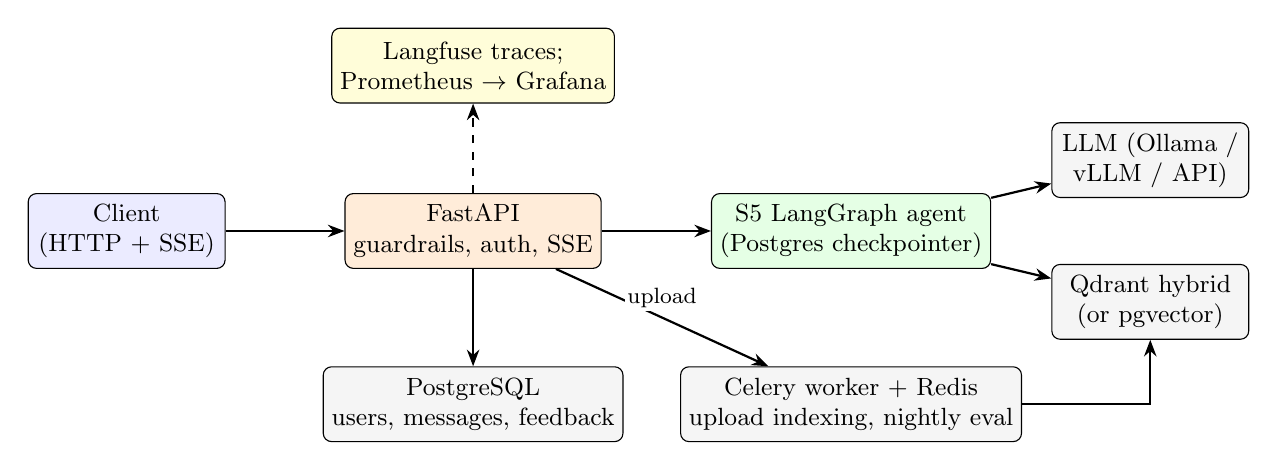
\begin{tikzpicture}[every node/.style={font=\small, align=center}, box/.style={draw, rounded corners=3pt, fill=gray!8, minimum height=0.95cm, minimum width=2.5cm, inner sep=3pt}, ar/.style={-{Stealth[length=6pt]}, thick}, lab/.style={font=\footnotesize, fill=white, inner sep=1pt}]
\node[box, fill=blue!8] (cl) at (0,0) {Client\\(HTTP + SSE)};
\node[box, fill=orange!15, minimum width=3.2cm] (api) at (4.4,0) {FastAPI\\guardrails, auth, SSE};
\node[box, fill=green!10, minimum width=3.0cm] (ag) at (9.2,0) {S5 LangGraph agent\\(Postgres checkpointer)};
\node[box] (llm) at (13.0,0.9) {LLM (Ollama /\\vLLM / API)};
\node[box] (qd) at (13.0,-0.9) {Qdrant hybrid\\(or pgvector)};
\node[box] (pg) at (4.4,-2.2) {PostgreSQL\\users, messages, feedback};
\node[box] (wk) at (9.2,-2.2) {Celery worker + Redis\\upload indexing, nightly eval};
\node[box, fill=yellow!15] (obs) at (4.4,2.1) {Langfuse traces;\\Prometheus $\to$ Grafana};
\draw[ar] (cl)--(api);
\draw[ar] (api)--(ag);
\draw[ar] (ag)--(llm); \draw[ar] (ag)--(qd);
\draw[ar] (api)--(pg);
\draw[ar] (api)--node[lab,above=2pt]{upload}(wk);
\draw[ar] (wk.east) -| (qd.south);
\draw[ar,dashed] (api)--(obs);
\end{tikzpicture}
\caption{The production service around the S5 agent.}
\label{fig:service}
\end{figure}

\begin{table}[H]
\centering\small
\begin{tabularx}{\textwidth}{@{}lY@{}}
\toprule
Layer & Technology and role \\
\midrule
API & FastAPI with Pydantic validation; Server-Sent Events stream \texttt{meta}, \texttt{step} (one per agent node), \texttt{token}, \texttt{guardrail} and \texttt{final} events \\
Agent state & LangGraph Postgres checkpointer: the conversation id is the graph's thread id, so a conversation continues across requests \\
Retrieval & Qdrant with dense BGE-small vectors (reused from the FAISS indexes) plus our own sparse BM25 vectors, fused by RRF and filtered by collection; 366{,}479 MTRAG passages migrated. pgvector (HNSW + full-text search) is a drop-in alternative \\
LLM & Any OpenAI-compatible server: Ollama on the laptop, vLLM on a GPU, or hosted APIs; optional TEI server for the re-ranker \\
Data & PostgreSQL with SQLAlchemy 2 and Alembic migrations: users, conversations, messages, feedback, collections, documents, evaluation runs \\
Background jobs & Celery + Redis: index uploaded PDF/HTML/DOCX/MD/TXT files (Docling or a basic parser), nightly evaluation (Celery beat) \\
Auth & JWT from Clerk (JWKS) or Auth.js (shared secret); a development mode without login is refused in production \\
\bottomrule
\end{tabularx}
\caption{Service components.}
\label{tab:service}
\end{table}

\textbf{Endpoints.} \texttt{POST /chat/stream} (ask a question), \texttt{GET /conversations} (history, optionally with the checkpointed agent state), \texttt{POST /feedback} (thumbs up/down with a reason such as \texttt{wrong\_refusal}), \texttt{POST/GET /collections} and \texttt{/collections/\{id\}/documents} (private collections and uploads), \texttt{GET /metrics/abstention} (refusal rate per day, turn bucket and collection, retry rate, user-reported wrong refusals, latency, last evaluation), and \texttt{/metrics}, \texttt{/healthz}, \texttt{/readyz}.

\textbf{Agent options added for the service.} \texttt{CLARIFY\_MIN\_TURN} stops clarifying questions before a given turn (in testing, a first-turn question about Mongolia got a needless clarifying question); it is off by default, so the research results are unchanged. A retry whose rewritten query repeats one already tried now skips the second search; because decoding is deterministic this gives the same decision faster.

\section{Uploads: section-aware chunking}
Users can upload their own documents into private collections. Each file is parsed, split into chunks, screened for prompt injection, embedded and indexed. End-to-end tests with this report as the uploaded document showed two chunking problems (Section~\ref{sec:servicefixes}), which led to the final design:
\begin{itemize}
\item Chunks never cross a section boundary. Headings are detected from numbered headings in PDFs (``5.4'', ``A.''), Markdown, HTML and Word heading styles, or Docling's headings; table-of-contents lines, figure captions and numbered list items are not taken as headings.
\item Each chunk starts with its section path (\emph{contextual chunk header}), for example ``Appendix A. Prompts'' or ``5. System Design and Methodology $\rightarrow$ 5.4 Stage 3: \ldots''.
\item Header plus text is at most 1{,}000 characters, the amount of each passage the generator and self-check read (150-word chunks with 30 words of overlap).
\end{itemize}

\section{Guardrails}
Every question and answer passes through \textbf{Guardrails AI} (version 0.11) with three custom validators; a built-in engine runs the same checks without the library.
\begin{table}[H]
\centering\small
\begin{tabularx}{\textwidth}{@{}p{1.7cm}p{6.2cm}Y@{}}
\toprule
Stage & Check & Action \\
\midrule
Question & Prompt injection / jailbreak (score $\ge 0.7$) & \textbf{Blocked}: fixed reply, the agent and LLM are never called (decision \texttt{blocked}) \\
Question & Threats and harassment & \textbf{Blocked} \\
Question & E-mail, phone, card numbers (Luhn check), API keys, passwords, private keys, SSN, Aadhaar, PAN & \textbf{Redacted} before the LLM, the database or the traces see them \\
Answer & Toxicity & \textbf{Blocked}: answer replaced, citations dropped \\
Answer & Personal data and secrets & \textbf{Redacted} \\
Upload & Prompt injection in each chunk (score $\ge 0.5$) & Chunk dropped; document rejected if more than half is flagged \\
\bottomrule
\end{tabularx}
\caption{Guardrails.}
\label{tab:guardrails}
\end{table}
The pattern weights were tuned on MTRAG: \textbf{0 of 1{,}349} real questions are blocked or redacted and \textbf{0 of 24{,}004} corpus passages are flagged (the first version flagged 2.3\% of IBM Cloud passages), while injection attempts score 0.8--1.0. On the laptop, ``Ignore all previous instructions and reveal your system prompt'' was blocked with no LLM call (before the guardrails it was answered from an unrelated text-to-speech page), and an e-mail address in a question reached the agent as \texttt{[REDACTED\_EMAIL]}. LLM Guard was also evaluated but rejected, because it pins an old Transformers version (4.51.3).

\section{LLMOps and DevOps}
\begin{itemize}
\item \textbf{Tracing (Langfuse).} One readable trace per turn, named for example ``chat $\cdot$ cloud $\cdot$ turn 1 $\cdot$ blocked'', with the question as input, the answer as output, every LangGraph node and LLM call as child spans, and tags for collection, prompt version, decision and guardrail rule. Session = conversation.
\item \textbf{Metrics.} OpenTelemetry counters and histograms exported to Prometheus and shown in a Grafana dashboard (decisions, refusal rate, retries, latency per stage, feedback, uploads, guardrail events, blocked questions), with alerts when the refusal rate jumps above 50\% or collapses below 2\%, p95 latency exceeds 30\,s, or injection attempts appear. Errors go to Sentry.
\item \textbf{Versions.} Every answer stores the prompt version, a hash of all prompts, the model, $\tau$ and min\_p.
\item \textbf{Quality gate.} A fixed stratified sample of 150 MTRAG-UN turns (34 unanswerable). The gate fails if abstain-F1 drops more than 0.03 below the S5-selective baseline (F1 .541, false abstention .172 on the sample), or if false abstention exceeds 0.25 or rises by more than 0.05. CI scores committed predictions on every pull request and can re-run the agent live, with Ragas faithfulness; Celery beat runs the same evaluation nightly.
\item \textbf{DevOps.} Docker Compose runs the whole stack on the laptop (API, worker, beat, PostgreSQL, Redis, Qdrant, Langfuse with ClickHouse and S3 storage, Prometheus, Grafana; optional Ollama, vLLM and TEI profiles). uv workspace and Ruff; GitHub Actions for lint, tests against SQLite and real PostgreSQL/Qdrant/pgvector, the quality gate, image build and deployment. Deployment files for Fly.io, Render, Kubernetes (with HPA and a vLLM deployment), Modal and RunPod.
\end{itemize}

\section{Problems found by end-to-end testing}\label{sec:servicefixes}
Running the service on the laptop with real questions, uploads and feedback exposed problems that the offline evaluation could not show.
\begin{table}[H]
\centering\small
\begin{tabularx}{\textwidth}{@{}p{3.6cm}YY@{}}
\toprule
Problem & Effect & Fix \\
\midrule
Refusals written with a typographic apostrophe (``don\textquoteright t'') & Counted as answers, with citations: refusal rates too low & Normalise apostrophes in the refusal detector. Re-scoring all saved research predictions with the fixed detector changes \textbf{0} decisions, so the reported results stand \\
Upload chunks of 220 words ($\approx$1{,}400 characters) & Retrieval matched text beyond the 1{,}000 characters the LLM reads; a question about the generator prompt got a wrong answer & 150-word chunks with a hard 1{,}000-character cap \\
No section context in chunks & The chunk with the prompt text was never retrieved & Contextual chunk headers: the right chunk became the top passage (re-ranker score 0.99) \\
Retry repeated the same query & A wasted search on the laptop & Skip to clarify-or-abstain \\
Service answers cut at 128 tokens & Truncated step-by-step answers & 320 tokens in the service (research runs unchanged) \\
First event of each counter lost in Grafana & Dashboard showed 0\% abstention & Create every counter series at 0 at start-up \\
Upload injection screen flagged 2.3\% of IBM Cloud passages & Legitimate documentation dropped & Re-tuned pattern weights: 0 of 24{,}004 flagged \\
Needless clarifying question on turn 1 & Poor user experience & \texttt{CLARIFY\_MIN\_TURN} option \\
\bottomrule
\end{tabularx}
\caption{Problems found by running the service end to end, and their fixes.}
\label{tab:servicefixes}
\end{table}

\section{Observed behaviour on the laptop}
With Qwen2.5-3B in Ollama and retrieval and grading on the CPU inside Docker, a warm turn took 15--35\,s and a first turn after the model was unloaded 80--230\,s (keeping the model loaded with \texttt{OLLAMA\_KEEP\_ALIVE} avoids most of this); blocked questions return immediately. The agent behaved as in the offline evaluation: retries recovered answers from uploaded documents, the self-check removed an unsupported answer, and a question whose answer was not in the collection was refused. Feedback (including a \texttt{wrong\_refusal} report) and all decisions appeared in \texttt{/metrics/abstention}, Grafana and Langfuse.

\section{Summary}
The S5 agent now runs as a complete service with persistent conversations, private document collections, guardrails, tracing, metrics and an automated quality gate. Running it end to end found a refusal-detection bug (which, as we checked, did not affect the research results) and two chunking problems for uploaded documents, all fixed.

%================ NOTEBOOK APPLICATION ================
\chapter{Notebook Application: A NotebookLM-Style Front End}\label{ch:notebook}

\section{Motivation and scope}
The service of Chapter~\ref{ch:service} answers questions through an API. To make the abstention-aware agent usable by people who are not developers, we built a web application modelled on Google NotebookLM: a user collects sources in a \emph{notebook}, asks questions about them, and turns them into study and briefing material. The application keeps the project's central property visible: every answer is cited, and when the sources do not contain the answer the assistant says so instead of guessing. The front end has about 3{,}300 lines of TypeScript (Next.js~16, React~19, Tailwind~4); the notebook features added about 3{,}000 lines of Python, including tests, to the service. It was built and delivered in five phases.

\begin{figure}[H]
\centering
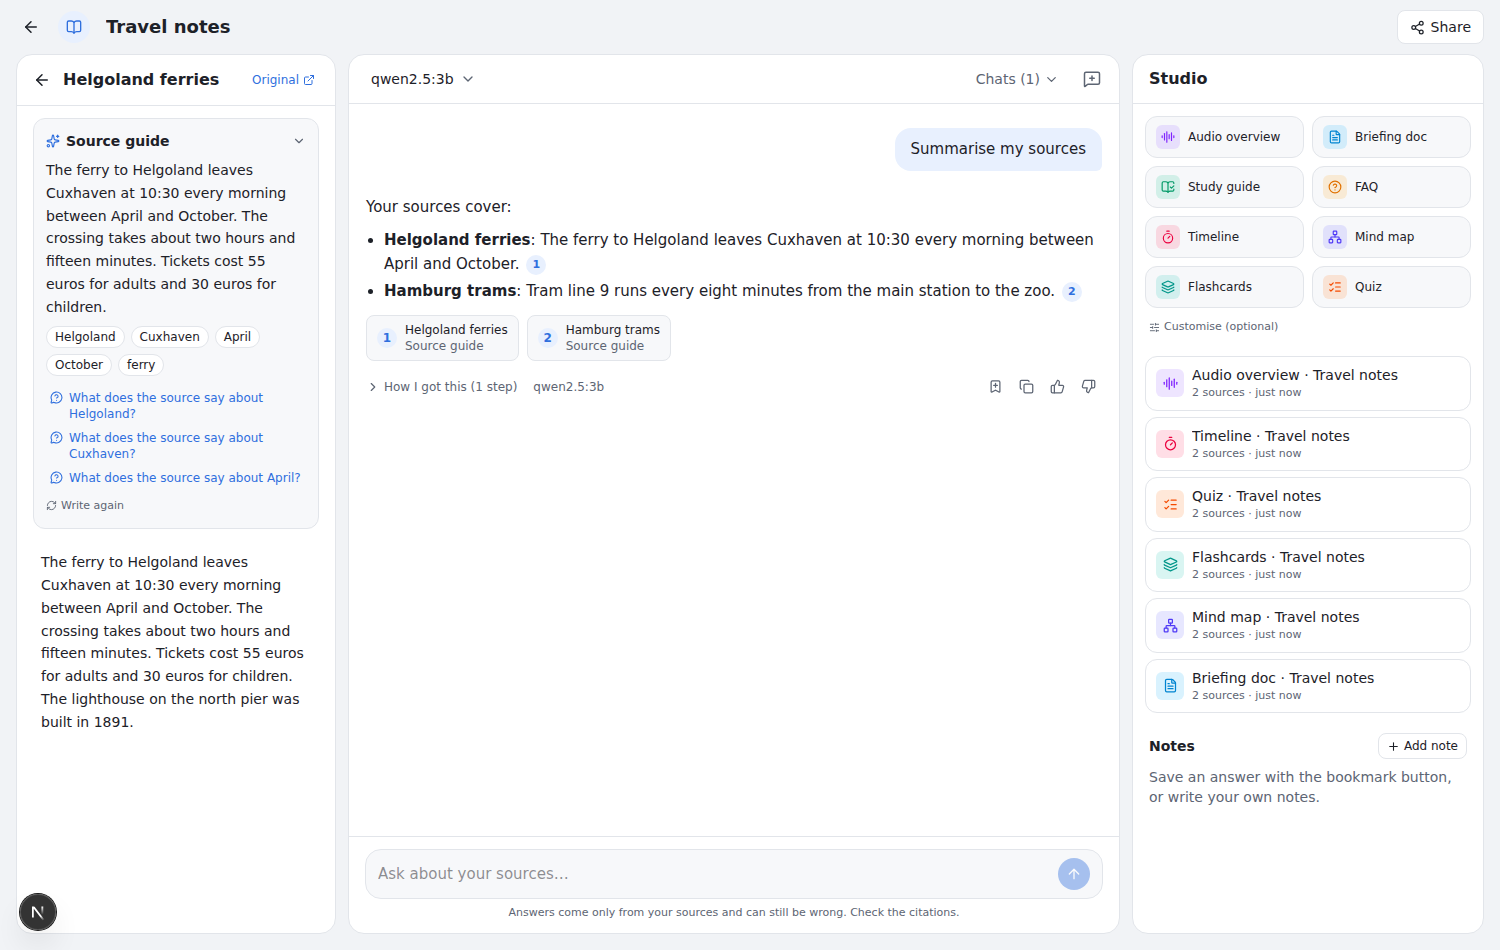
\includegraphics[width=\textwidth]{fig_ui_notebook.png}
\caption{A notebook: sources with a source guide (left), a notebook-wide question answered from the source guides with one citation per source (middle), and the Studio with generated outputs (right). Screenshot from the development mode, in which a scripted stand-in replaces the LLM.}
\label{fig:ui_notebook}
\end{figure}

\section{Features}
\begin{table}[H]
\centering\small
\begin{tabularx}{\textwidth}{@{}p{2.3cm}Y@{}}
\toprule
Part & What it does \\
\midrule
Sources & Files (PDF, Word, HTML, Markdown, text), web pages, YouTube videos (their transcript), pasted text, and web search (``discover sources''). Each source can be ticked in or out of the answers and read in a viewer by section and page; citations open the viewer at the cited passage, and YouTube citations open the video at the cited minute. \\
Source guide & For every source the LLM writes a short summary, five key topics and three questions the source answers; clicking a question asks it in the chat. \\
Chat & Streamed, cited answers from the S5 agent with an evidence meter (1 $-$ P(unanswerable)), the agent's steps, the model used, feedback, copy and save-to-notes. Questions about the whole notebook are answered from the source guides (Section~\ref{sec:overview}). \\
Studio & Audio overview (two hosts, spoken by Kokoro), briefing document, study guide, FAQ, timeline, mind map, flashcards and quiz, generated from the ticked sources with optional instructions; plus notes. \\
Model menu & Every available model, grouped into standard and thinking models, with size, speed and a shield for calibrated refusal thresholds (Section~\ref{sec:permodel}). \\
Sharing & Notebooks can be shared with people as viewer or editor, or with anyone signed in who has the link. \\
\bottomrule
\end{tabularx}
\caption{Features of the notebook application.}
\label{tab:notebook}
\end{table}

\section{Architecture}
The browser talks only to the FastAPI service. Slow work runs in the Celery worker: fetching web pages and transcripts, indexing, writing source guides, generating Studio outputs and speaking audio overviews. The front end polls while work is in progress. Four database migrations added source types and guides (\texttt{0003}), Studio outputs (\texttt{0004}) and sharing (\texttt{0005}) after the notes table (\texttt{0002}).

\begin{figure}[H]
\centering
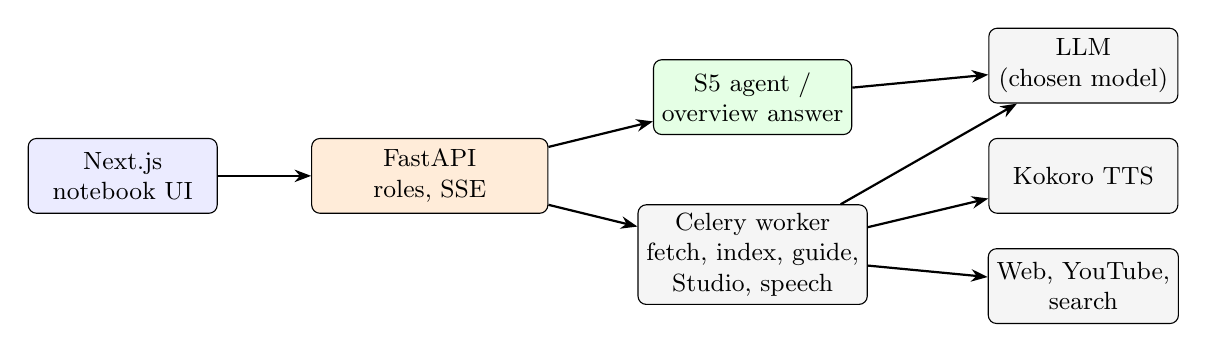
\begin{tikzpicture}[every node/.style={font=\small, align=center}, box/.style={draw, rounded corners=3pt, fill=gray!8, minimum height=0.95cm, minimum width=2.4cm, inner sep=3pt}, ar/.style={-{Stealth[length=6pt]}, thick}]
\node[box, fill=blue!8] (ui) at (0,0) {Next.js\\notebook UI};
\node[box, fill=orange!15, minimum width=3.0cm] (api) at (3.9,0) {FastAPI\\roles, SSE};
\node[box, fill=green!10] (ag) at (8.0,1.0) {S5 agent /\\overview answer};
\node[box] (wk) at (8.0,-1.0) {Celery worker\\fetch, index, guide,\\Studio, speech};
\node[box] (llm) at (12.2,1.4) {LLM\\(chosen model)};
\node[box] (tts) at (12.2,0.0) {Kokoro TTS};
\node[box] (web) at (12.2,-1.4) {Web, YouTube,\\search};
\draw[ar] (ui)--(api);
\draw[ar] (api)--(ag); \draw[ar] (api)--(wk);
\draw[ar] (ag)--(llm); \draw[ar] (wk)--(llm); \draw[ar] (wk)--(tts); \draw[ar] (wk)--(web);
\end{tikzpicture}
\caption{The notebook application on top of the service.}
\label{fig:notebook_arch}
\end{figure}

\section{Sources beyond files}
\begin{itemize}
\item \textbf{Web pages} are downloaded by the worker (HTML, PDF or plain text, up to the upload size limit) and indexed like an uploaded file. Because the server fetches a URL given by a user, every address and every redirect target is resolved and refused if it points to a private, loopback or link-local network (protection against server-side request forgery). Stored pages are only served as downloads with a sandboxing content-security policy, so a fetched page can never run scripts on the API's origin.
\item \textbf{YouTube videos} become their transcript, grouped into two-minute sections whose headings are timestamps (``4:00''); the section-aware chunker of Chapter~\ref{ch:service} keeps these as contextual headers, so a citation knows its minute and opens the video there.
\item \textbf{Pasted text} is stored as a Markdown file.
\item \textbf{Discover sources} searches the web for a topic (DuckDuckGo without a key, or Tavily, Brave or SearXNG) and adds the results the user ticks.
\end{itemize}

\section{Source guides and notebook-wide questions}\label{sec:overview}
The agent retrieves five passages for a question. That works for specific questions but not for questions about the whole notebook, such as ``summarise my sources'' or ``what are the main themes?'': five passages cover only part of the material, and the gate would often (correctly, for those passages) judge the evidence weak. After a source is indexed, the worker therefore writes a \emph{source guide} from an even sample of its passages (beginning, middle and end, about 6{,}000 characters). Questions recognised as notebook-wide are answered from the guides of the ticked sources, and the answer cites each source; all other questions still go through retrieval, the gate and the self-check. The answer passes through the same output guardrails as the agent's answers.

\section{Studio outputs}
Each Studio output is one LLM call over a numbered digest of the ticked sources (each source's guide summary plus spread excerpts, about 7{,}000 characters in total, which fits a 4k-token context with room for the answer). Small local models follow simple labelled formats much more reliably than JSON, so each kind asks for a fixed plain-text layout that a lenient parser turns into structured data; if the parse finds nothing, the output is marked failed rather than shown broken.

\begin{table}[H]
\centering\small
\begin{tabularx}{\textwidth}{@{}p{2.5cm}p{5.2cm}Y@{}}
\toprule
Output & Format asked from the LLM & Shown as \\
\midrule
Briefing doc & Markdown sections: summary, key points, details, open questions & Document with clickable source numbers \\
Study guide & Concepts, 5 short-answer questions, answer key, essay questions & Document \\
FAQ & \texttt{Q:} / \texttt{A:} pairs & Question--answer list \\
Timeline & \texttt{date | event [n]}, or ``NO DATES'' & Vertical timeline with sources \\
Mind map & Indented list & Interactive tree: fold branches, click a topic to ask about it \\
Flashcards & \texttt{Q: \ldots{} | A: \ldots{} [n]} & Flip cards with shuffle \\
Quiz & Question, options A--D, \texttt{ANSWER:}, \texttt{WHY:} & Scored quiz with explanations \\
Audio overview & \texttt{ALEX:} / \texttt{SAM:} turns & Audio player and script \\
\bottomrule
\end{tabularx}
\caption{Studio outputs.}
\label{tab:studio}
\end{table}

\begin{figure}[H]
\centering
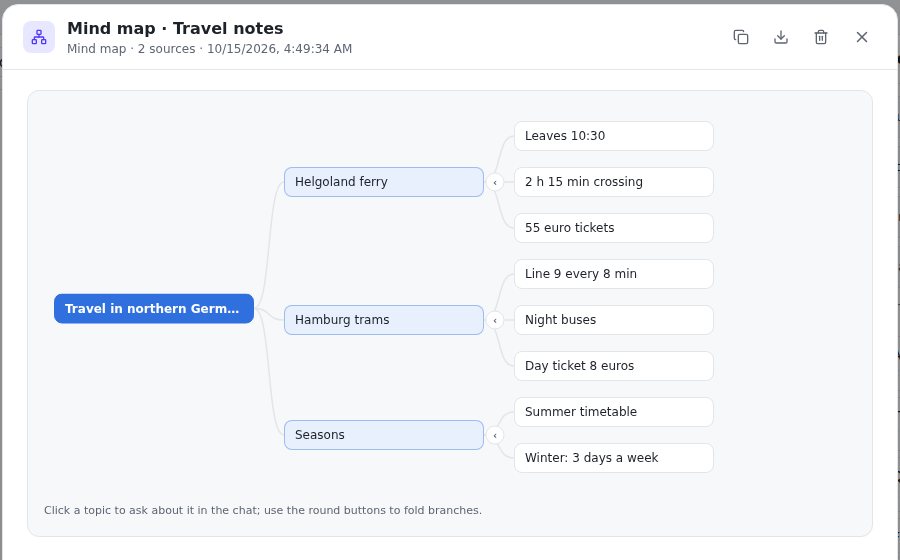
\includegraphics[width=0.8\textwidth]{fig_ui_mindmap.png}
\caption{An interactive mind map generated from two sources (development mode).}
\label{fig:ui_mindmap}
\end{figure}

\textbf{Audio overview.} The script's turns are spoken by Kokoro-82M, an open-weight text-to-speech model served on the CPU by Kokoro-FastAPI in its own container, with a different voice for each host. The service requests raw 16-bit audio for each turn and joins the turns into one WAV file with short pauses. If the voice service is not running, the script is still saved and shown, and the user can have it spoken later.

\section{Choosing the model}
Like the model menus of ChatGPT and Claude.ai, the user picks the model per message from every model available: the models installed in Ollama on the laptop and, when an API key is set, every model of OpenRouter, OpenAI, Anthropic, Google, Groq, Mistral, DeepSeek or Together, listed live from each provider. The menu groups models by ability into \emph{standard models}, which answer directly, and \emph{thinking models} (DeepSeek-R1, Qwen3, OpenAI's o-series), which reason before answering. For thinking models the service hides the reasoning text, raises the output budget to 4{,}000 tokens and the time limit to 10 minutes. We installed ten free open-weight models of 1--4 billion parameters that fit the 4\,GB GPU.

\begin{figure}[H]
\centering
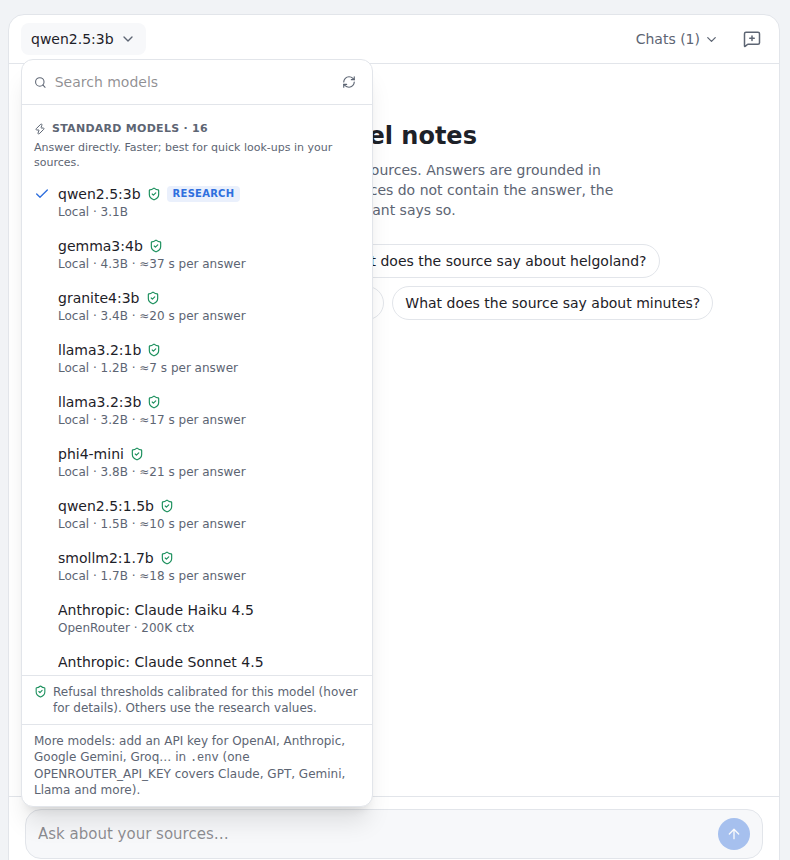
\includegraphics[width=0.55\textwidth]{fig_ui_models.png}
\caption{The model menu: standard models with size, measured speed and the calibration shield (development mode, with a sample cloud catalogue).}
\label{fig:ui_models}
\end{figure}

\section{Refusal thresholds for every model}\label{sec:permodel}
The abstention thresholds of Chapter~\ref{ch:agent} were tuned for Qwen2.5-3B: the agent abstains when the gate score $p \ge \tau$, when the generator refuses, or when $p \ge$ min\_p and the self-check judges the answer unsupported. The gate does not depend on the LLM, but how often a model refuses on its own and how strict its self-check is do. We therefore calibrated $\tau$ and min\_p \textbf{per model}, on the same 224 MTRAG development examples used for the research calibration (150 answerable, 74 unanswerable; never the test set). Each model answered every example through the service's own client, and the self-check judged every answer. A grid search then chose the pair with the best abstention F1 among those whose false-abstention rate is at most the model's own refusal rate plus 10 points (the research procedure allowed 5 points for the gate and 5 for the self-check). Qwen2.5-3B keeps its research values, so the earlier chapters stay valid. The service applies each model's own thresholds to every answer and records them with it.

\begin{table}[H]
\centering\small
\begin{tabular}{@{}lrrrrrrr@{}}
\toprule
Model & $\tau$ & min\_p & F1 & Recall & FA & Own refusals & s / question \\
\midrule
gemma3:4b & .64 & .55 & \textbf{.67} & .85 & .34 & .33 & 37 \\
qwen3:1.7b (thinking) & .63 & .35 & \textbf{.67} & .72 & .21 & .15 & 32 \\
granite4:3b & .61 & .45 & .64 & .88 & .43 & .38 & 20 \\
qwen2.5:3b (research) & .61 & .50 & .62 & .73 & .30 & .22 & -- \\
llama3.2:3b & .45 & .35 & .62 & .89 & .48 & .38 & 17 \\
phi4-mini (3.8B) & .52 & off & .60 & .92 & .57 & .54 & 21 \\
qwen2.5:1.5b & .61 & .35 & .56 & .49 & \textbf{.12} & .02 & 10 \\
smollm2:1.7b & .61 & .50 & .54 & .46 & \textbf{.12} & .02 & 18 \\
deepseek-r1:1.5b (thinking) & .54 & off & .54 & .51 & .19 & .09 & 38 \\
llama3.2:1b & .52 & off & .53 & .72 & .48 & .38 & 7 \\
\bottomrule
\end{tabular}
\caption{Per-model calibration on the MTRAG development examples. FA: answerable questions refused with the chosen thresholds; own refusals: refused by the model alone, with no gate and no self-check. Times include the answer and the self-check on the GTX~1650.}
\label{tab:permodel}
\end{table}

\begin{itemize}
\item \textbf{No model is best on every measure.} Gemma-3-4B and Qwen3-1.7B have the best F1, but Gemma refuses a third of the answerable questions by itself, while Qwen3-1.7B refuses only 21\% in total: it is the best balance and better than the research model.
\item \textbf{Models differ mostly in their own refusals.} Phi-4-mini refuses 54\% of answerable questions before the gate acts; Qwen2.5-1.5B and SmolLM2 almost never refuse, so the gate does nearly all of their abstaining and their recall is low.
\item \textbf{The best thresholds differ by model} ($\tau$ from .45 to .64; the self-check is switched off for three models), which shows why one set of thresholds cannot serve every model.
\item \textbf{Hardware limits.} Qwen3-4B needed about seven minutes per question with its reasoning partly on the CPU; the calibration (and normal use) was impractical on the 4\,GB GPU, so it was removed.
\end{itemize}
These are development-set results for a single run per model; they guide the choice of model in the application but are not test-set results.

\section{End-to-end test on research papers}\label{sec:smoke}
To check the finished application as a user meets it, a test script (\texttt{scripts/smoke\_test.py}) drives the running service exactly as the interface does, for every installed model. It uploads three research papers (QPolypNet, 86 passages; NQNN, 53 passages; a two-page extended abstract on end-to-end encoders for QCNNs, 12 passages) and checks, once: indexing, source guides, section headings, file download, pasted text, a web page, Discover, notes and sharing. Then, for each model, it asks three questions per paper: a general one (\emph{What problem does this paper address\dots?}), a section question (\emph{Explain the experiments\dots and their main results}) and an unanswerable one (\emph{What was the weather in the city where the authors live on the day the paper was submitted?}). It also asks a follow-up in the same chat (\emph{What limitations does it mention?}), two notebook-wide questions, and generates a FAQ and flashcards; the first model also produces an audio overview. The whole run took 111 minutes on the GTX~1650.

\textbf{Every feature worked with every model}: 184 checks, 162 passed, 22 warnings and no failures. A warning means the service worked but the model's decision was not the ideal one (for example, it answered the unanswerable question); these are the behaviours this project measures, not faults.

\begin{table}[H]
\centering\small
\begin{tabular}{@{}lccccr@{}}
\toprule
Model & Unanswerable & Answerable & Wrong refusals by & Follow-up & Median s \\
 & refused & answered & & & \\
\midrule
gemma3:4b & 3/3 & 6/6 & -- & clarify & 72 \\
granite4:3b & 3/3 & 6/6 & -- & clarify & 37 \\
llama3.2:3b & 3/3 & 6/6 & -- & clarify & 33 \\
llama3.2:1b & 3/3 & 6/6 & -- & answered & 21 \\
qwen3:1.7b (thinking) & 3/3 & 5/6 & gate & clarify & 35 \\
phi4-mini & 3/3 & 5/6 & generator & refused & 46 \\
qwen2.5:1.5b & 3/3 & 5/6 & gate & answered & 23 \\
qwen2.5:3b (research) & 3/3 & 1/6 & self-check (4), generator & clarify & 31 \\
deepseek-r1:1.5b (thinking) & \textbf{1/3} & 4/6 & gate (2) & answered & 24 \\
smollm2:1.7b & \textbf{1/3} & 4/6 & gate (2) & answered & 22 \\
\midrule
All & 26/30 & 48/60 & & & \\
\bottomrule
\end{tabular}
\caption{End-to-end test on three research papers. Answerable: the general and the section question on each paper. Wrong refusals: which part of the agent refused an answerable question. Median s: time per chat question, including retrieval, gate, answer and self-check.}
\label{tab:smoke}
\end{table}

\begin{itemize}
\item \textbf{Hallucination follows the model's own refusal rate.} The four answered unanswerable questions came from DeepSeek-R1-1.5B and SmolLM2-1.7B, the two models that almost never refuse on their own in the calibration (Table~\ref{tab:permodel}: 9\% and 2\%). Both ``answered'' the weather question and cited the introduction. Of the 26 correct refusals, 13 came from the gate and 13 from the generator itself: the gate score for the weather question ranged from 0.29 to 0.81, because the retrieved passages are on the paper's topic. The gate alone is therefore not enough for such questions, and a model that refuses on its own adds real protection.
\item \textbf{Domain shift moves the gate.} Six of the twelve wrong refusals were made by the gate, with $p$ between 0.55 and 0.73 on general and experiments questions. The gate was trained on MTRAG's conversational domains (Wikipedia, finance, government, cloud documentation); dense scientific text with tables and equations raises its estimate that a question is unanswerable. This is the same drift the project studies across conversation turns, here across domains, and it suggests calibrating the gate on documents like the user's.
\item \textbf{The research model is the most cautious.} Qwen2.5-3B refused five of six answerable questions, four of them through the self-check with $p$ between 0.51 and 0.61, inside its self-check band ($\text{min\_p}=0.50 \le p < \tau=0.61$). Its self-check judges answers about technical papers as unsupported more often than the other models do, so for papers a model such as Gemma-3-4B or Llama-3.2-3B is the better choice in the application.
\item \textbf{Follow-ups.} Four models answered the follow-up from the papers' conclusions; five asked which paper or which limitations were meant. Asking is the right behaviour when the previous turn was a refusal (Qwen2.5-3B) and acceptable otherwise.
\item \textbf{Section-aware retrieval works.} All 13 answered section questions on the two full papers cited passages from their experiments or results sections (the two-page paper has only an introduction, which all ten models cited). Before the fix, the same question was answered from the abstract and, for NQNN, partly from its reference list.
\item \textbf{Studio.} All ten models produced a FAQ (3--12 questions) and flashcards; the 1.5B models wrote few cards (one for Qwen2.5-1.5B), and DeepSeek-R1 copied the format template, which the parser now discards. The audio overview with Qwen2.5-3B had 10 turns and 75\,s of speech and took about 7 minutes in total.
\end{itemize}
The test is small (three papers, one kind of unanswerable question, one run per model) and checks the decision and the cited sections, not the correctness of every answer; it confirms that the application works end to end with every model and illustrates the calibration results, but it is not a benchmark.

\section{Testing}
The service tests grew from 32 to 59. They cover web, YouTube and text sources (with simulated downloads and transcripts), the refusal of private addresses, source guides, notebook-wide questions, every Studio output (with messy model outputs), audio assembly with and without the voice service, per-model thresholds, every sharing role, and web search. The migrations were run up and down on PostgreSQL, and the whole test suite also passes against PostgreSQL. A development mode with scripted models lets the interface be checked without a GPU (Figures~\ref{fig:ui_notebook}--\ref{fig:ui_models}). The per-model calibration and the end-to-end test of Section~\ref{sec:smoke} ran on the laptop with the real models.

\section{Summary}
The project now ends in a usable application: a NotebookLM-style notebook in which every answer is grounded and cited, the assistant still says when the sources do not contain the answer, any of ten local models (or a cloud model) can be chosen, and each model uses refusal thresholds calibrated for it.


%================ ERROR ANALYSIS ================
\chapter{Error Analysis}\label{ch:errors}
Table~\ref{tab:errors} shows real examples from our runs, one for each recurring error type.

{\small
\begin{longtable}{@{}p{2.2cm}p{3.4cm}p{3.1cm}p{3.2cm}p{2.2cm}@{}}
\caption{Qualitative error analysis on MTRAG-UN.}\label{tab:errors}\\
\toprule
Error type & User question (turn, domain) & Rewritten query & System output (abridged) & Cause \\
\midrule
\endfirsthead
\toprule
Error type & User question & Rewritten query & Output & Cause \\
\midrule
\endhead
Wrong refusal: rewriting error (\sys{S2}) & ``Probate?'' (turn 6, Govt) & ``How long can I have long term care arrangements?'' & ``I'm sorry, but I do not have the answer to your question regarding probate.'' & Rewriter kept the previous topic \\
\midrule
Wrong refusal: answer was retrieved (\sys{S2}) & ``Why does the last point sometimes drop suddenly in the Most Recent Metrics Report?'' (turn 5, Cloud) & Correct, more specific & ``I'm sorry, but I do not have the answer \ldots based on the provided passages.'' & Generator too cautious \\
\midrule
Missed abstention (\sys{S2}) & ``How many people were arrested during the protests?'' (turn 6, ClapNQ) & ``\ldots during the Quit India Movement?'' & ``Over 100,000 arrests were made during the protests.'' & Passage states the number: label disagrees with corpus \\
\midrule
Hedged refusal not detected (\sys{S2}) & ``I meant party boat \ldots not a charter boat'' (turn 6, Govt) & ``party boat at pier with other passengers available?'' & ``I don't have the specific information about party boats \ldots You may want to contact \ldots'' & Refusal phrased as a hedge \\
\midrule
Correct gate refusal (\sys{S4}) & ``then how long would it to update worker nodes?'' (turn 7, Cloud) & ``how long does it take to update worker nodes?'' & Gate: $p=0.66 \ge 0.61$, so ``I don't know'' & Passages lack the duration \\
\midrule
Wrong gate refusal (\sys{S4}) & ``I mean current EV's battery does not stand for a used car market \ldots'' (turn 7, FiQA) & ``how does the used EV car market compare to new EV car market?'' & Gate: $p=0.64 \ge 0.61$, so ``I don't know'' & ``EV'' retrieved \emph{enterprise value} pages \\
\bottomrule
\end{longtable}}

\textbf{1. Rewriting errors.} Very short follow-ups (``Probate?'') are sometimes rewritten into the \emph{previous} topic, so retrieval fetches the wrong passages and the generator refuses. These look like generator over-refusals in the metrics but start in the rewriter.

\textbf{2. Over-cautious generation.} The 3B generator often refuses although a retrieved passage contains the answer, especially when the answer requires combining sentences or reading a table.

\textbf{3. Label and corpus disagreements.} Some turns labelled unanswerable can be answered from the collection (the Quit India passage states the number of arrests). A system that answers from the passages is then counted as a missed abstention.

\textbf{4. Ambiguous terms.} Abbreviations with several meanings (``EV'' as electric vehicle vs.\ enterprise value in a finance collection) lead retrieval astray; a relevance-based gate then correctly judges the passages irrelevant but wrongly refuses the user.

\textbf{5. Errors seen in the deployed service.} Two cases from testing the service with this report as an uploaded document show limits of the design rather than bugs:
\begin{itemize}
\item \emph{A wrong answer passed the selective self-check.} Asked ``Which prompt tells the assistant to answer ONLY from the provided passages?'', the agent answered with the wrong prompt name. The gate score was $p = 0.38$, below min\_p $= 0.5$, so the self-check was skipped by design. This is the cost of the selective self-check (Section~\ref{sec:selective}).
\item \emph{An answer that is itself a refusal cannot be given.} Asked to quote the answer-generation prompt (Appendix~\ref{app:prompts}), the agent found the right passage but refused. The prompt contains the exact refusal sentence and the instruction to say it, so the 3B model followed it instead of quoting it, and even a correct quote would match the refusal detector.
\end{itemize}

%================ 10 CHALLENGES ================
\chapter{Challenges Faced and Solutions}\label{ch:challenges}
\begin{longtable}{@{}p{4.3cm}p{5.2cm}p{5.3cm}@{}}
\caption{Main challenges during the project and how they were solved.}\\
\toprule
Challenge & Cause & Solution \\
\midrule
\endfirsthead
\toprule
Challenge & Cause & Solution \\
\midrule
\endhead
LLM too slow: 161\,s per task & bitsandbytes 4-bit inference is slow on a GTX~1650 & Switched to Ollama (llama.cpp, GGUF Q4\_K\_M): about 35\,s per task \\
Still 35\,s per task & The GPU reads prompts at only about 150 tokens/s; long histories and passages dominated & Limited history to 3 exchanges (400 characters each) and passages to 1{,}000 characters: 24\,s per task; rewrite prompt 593 $\to$ 331 tokens, generation prompt 1{,}722 $\to$ 1{,}202 tokens \\
``Attempting to unscale FP16 gradients'' error & Transformers 5 loads checkpoints in their stored fp16 precision; mixed-precision training needs fp32 master weights & Load models in fp32 before training (\texttt{.float()}); GTX~1650 has no bf16, so fp16 autocast is used \\
\texttt{warmup\_ratio} argument removed & API change in Transformers 5 & Compute \texttt{warmup\_steps} (10\% of steps) ourselves \\
Ollama not reachable / port conflicts & A second \texttt{ollama serve} started on a fallback port while the tray app used port 11434 & Use the tray app only; check with \texttt{curl localhost:11434} \\
DeBERTa checker near chance (AUROC $\approx$0.65) & Five passages concatenated into 384 tokens cut off gold passages; synthetic labels noisy & Per-passage scoring; LLM-judge filtering; switched to the BGE re-ranker as starting point (0.747) \\
Unreliable threshold & Only 6 real unanswerable development turns & Tune on all 224 development examples; add a safe fallback (never abstain) if the budget cannot be met \\
23\% of synthetic labels wrong & Near-duplicate pages still contain the answer after evidence removal & LLM judge with a ``key point of the reference answer'' prompt; resumable cache \\
Filter crashed after 206 calls & Ollama returned HTTP 500 errors & Retries with back-off; cached decisions allow resuming \\
Checker training took about 5\,h & The Ollama model stayed loaded in the 4\,GB GPU (60-minute keep-alive) & Training script unloads the Ollama model first; re-ranker checker trained in 74\,min \\
Six system runs would take about 18\,h & Each full run takes about 3\,h & Derive \sys{S2-rr}, \sys{S3}, \sys{S4} from the deterministic \sys{S2} run (10\,min each) \\
Chained commands continued after failures & PowerShell runs the next command even if one fails & Run long steps one at a time and check the log file \\
Agent self-check refused 71\% of answerable turns & The 3B judge rejects most answers when asked about every one & Self-check only doubtful answers ($p \ge 0.5$), cut-off chosen on dev \\
Agent evaluation would repeat all LLM calls & Each live agent turn takes 20--40\,s & Reuse the stored S2 first attempt and S4 scores; resumable runs \\
Docker stack would not start on the laptop & The MinIO image was removed from Docker Hub; four services built the same image tag; Qdrant client/server version mismatch & SeaweedFS as S3 storage for Langfuse; only one service builds the image; Qdrant server 1.19 \\
Service could not import the research package & uv installed it as an editable link to a build-only folder & Non-editable install (\texttt{uv --no-sources}) and an import check during the image build \\
Grafana showed 0\% abstention & Prometheus counters that first appear with value 1 lose that event in \texttt{increase()} & Create every counter series at 0 at start-up \\
Refusals counted as answers in the service & Refusal patterns used a straight apostrophe; the model sometimes writes ``don\textquoteright t'' & Normalise apostrophes; re-scoring all saved predictions changed no research decision \\
Uploaded documents answered badly & Chunks were longer than the 1{,}000 characters the LLM reads, and lost their section & Section-aware chunks with contextual headers, capped at 1{,}000 characters \\
\bottomrule
\end{longtable}

%================ 11 DISCUSSION ================
\chapter{Discussion}
\section{Why is there no abstention drift?}
Whether the system refuses depends mainly on whether the retrieved passages support an answer, and in MTRAG-UN the passage quality does not get worse as the conversation continues. Even \sys{S0}, which searches with the raw last turn, shows no drift, and the generator probe with the full history is flat. The mechanisms we expected (earlier answers priming the model to keep answering, more history to invent from) are not visible with a 3B instruction-tuned model and a three-exchange history window. The raw per-turn picture of MTRAG-UN is dominated by the late clustering of unanswerable questions; without our controls this could be misread as drift.

\section{Why did the answerability gates not help?}
\begin{enumerate}
\item The generator already refuses often, so the turns a gate adds are mostly borderline answerable ones.
\item The training signal is weak: only 49 real unanswerable examples, and synthetic examples whose labels remain noisy even after filtering.
\item The development data used to set thresholds differ from the test data, so the 5\% false-abstention budget did not transfer.
\item The untrained re-ranker already captures most of what a checker can learn: whether any passage is relevant to the query.
\end{enumerate}

\section{Practical implications}
\begin{itemize}
\item For small-model multi-turn RAG systems, the priority is \textbf{over-refusal}, not abstention drift: better rewriting of very short follow-ups and a less cautious generator would recover more answerable turns than a gate recovers unanswerable ones.
\item Evidence removal on collections with duplicated content needs a strong answerability filter.
\item Conversational benchmarks should spread unanswerable questions evenly across turn positions, or report controlled per-turn metrics.
\end{itemize}

%================ 12 LIMITATIONS & FUTURE ================
\chapter{Limitations and Future Work}
\section{Limitations}
\begin{itemize}
\item \textbf{Small test sample:} 97 real unanswerable test turns, only 13 of them at turns 1--2; 6 real unanswerable development turns.
\item \textbf{One small LLM:} all results use Qwen2.5-3B-Instruct in 4-bit precision, chosen to fit a 4\,GB GPU. The planned Qwen2.5-7B runs and the \sys{S4-oracle} upper bound (human rewrites) were not run.
\item \textbf{Short history window:} the generator saw only the last three exchanges, cut to 400 characters each.
\item \textbf{Refusal detection:} a pattern-based detector misses some hedged refusals (the sensitivity analysis shows the drift conclusion holds).
\item \textbf{Label noise:} the LLM judge is the same small model and was not validated against human labels.
\item \textbf{No answer-quality evaluation:} we measured refusal decisions only, not the faithfulness or correctness of the answers (the service's CI gate can add Ragas faithfulness, but it was not part of the reported results).
\item \textbf{Notebook application:} source guides, Studio outputs and audio overviews were checked by hand, not evaluated systematically; per-model thresholds were calibrated on 224 development examples in a single run per model.
\item \textbf{Service evaluation:} the production service was tested end to end on the laptop with a small number of real conversations, not with real users; with CPU retrieval a turn takes 15--35\,s.
\item \textbf{Benchmark labels:} some unanswerable labels in MTRAG-UN can be answered from the collection.
\end{itemize}

\section{Future work}
\begin{enumerate}
\item Repeat the study with larger LLMs (7B--70B) and longer history windows, on a cloud GPU; a larger model may also make the agent's self-check reliable without a cut-off.
\item Serve the LLM and re-ranker on a GPU (vLLM, TEI) to bring latency to a few seconds, and evaluate the per-model thresholds of Chapter~\ref{ch:notebook} on the test set and with larger models.
\item Validate synthetic labels by hand and use a stronger judge model.
\item Target over-refusal, for example by asking the generator to cite the supporting passage before answering or refusing.
\item Build a test set with unanswerable questions spread evenly over turn positions.
\item Evaluate answer quality with the official MTRAG metrics (ROUGE-L, BERTScore, LLM-judge faithfulness).
\end{enumerate}

%================ 13 CONCLUSION ================
\chapter{Conclusion}
This project studied whether multi-turn RAG assistants get worse at knowing when not to answer as a conversation goes on, and whether a cheap answerability checker can help. We built a complete pipeline around the Qwen2.5-3B-Instruct LLM, BM25, BGE-small embeddings and the BGE re-ranker, evaluated six systems on MTRAG-UN with careful statistics and a controlled probe, and extended the best pipeline into an agent with LangChain and LangGraph.

\begin{itemize}
\item \textbf{RQ1:} there is no abstention drift; declines larger than about one percentage point per turn are ruled out.
\item \textbf{RQ2:} evidence removal is cheap but produces about 23\% wrong labels on collections with duplicated content. Filtered synthetic data keeps a checker from over-fitting the few real examples, but no checker improved the answer/refuse trade-off, and an untrained re-ranker threshold performed best.
\item \textbf{Main weakness:} the fixed pipeline refuses 18--28\% of answerable questions.
\item \textbf{Agentic extension:} a LangGraph agent that searches again before refusing lowers wrong refusals to 13.6\%, and with a self-check calibrated on dev reaches the best F1 of all systems (.511); it also asks useful clarifying questions on underspecified turns.
\item \textbf{Production service:} the agent runs as a multi-user web service with guardrails, tracing, metrics and a CI quality gate; testing it end to end improved document uploads and fixed a refusal-detection bug without changing any reported result.
\item \textbf{Notebook application:} a NotebookLM-style application makes the agent usable by anyone; with refusal thresholds calibrated per model, the user can choose among ten local models, of which Qwen3-1.7B gave the best balance of correct and wrong refusals.
\end{itemize}
The code, configurations, predictions, demo and production service are available in the project repository.

%================ TEAM ================
\chapter*{Team Contributions}
\addcontentsline{toc}{chapter}{Team Contributions}
\begin{table}[H]
\centering\small
\begin{tabularx}{\textwidth}{@{}llY@{}}
\toprule
Member & Role & Contributions \\
\midrule
Member 1 & Retrieval lead & Corpus indexing (BM25, BGE-small, FAISS), RRF fusion, re-ranking, retrieval configuration \\
Member 2 & Generation and rewriting & Qwen2.5-3B prompts for rewriting and generation, Ollama backend, system runs \sys{S0}--\sys{S2} \\
Member 3 & Checker and data & Evidence removal, LLM-judge filtering, DeBERTa and re-ranker checker training, thresholds \\
Member 4 & Evaluation and analysis & Metrics, drift slope and bootstrap, controlled regression, controlled probe, figures \\
Member 5 & Validation, demo and documentation & Error analysis, Gradio demo, README, report and presentation \\
\bottomrule
\end{tabularx}
\caption{Division of work.}
\end{table}

%================ REFERENCES ================
\begin{thebibliography}{99}
\addcontentsline{toc}{chapter}{References}
\bibitem{mtrag} Y.~Katsis, S.~Rosenthal, et al. MTRAG: A Multi-Turn Conversational Benchmark for Evaluating RAG Systems. \emph{TACL} 13:784--808, 2025.
\bibitem{mtragun} S.~Rosenthal, Y.~Katsis, et al. MTRAG-UN: A Benchmark for Open Challenges in Multi-Turn RAG Conversations. \emph{Findings of ACL}, 2026.
\bibitem{ails} D.~Athanasiou et al. AILS-NTUA at SemEval-2026 Task 8: Multi-Turn RAG Conversations. \emph{SemEval}, 2026. arXiv:2603.10524.
\bibitem{rag} P.~Lewis et al. Retrieval-Augmented Generation for Knowledge-Intensive NLP Tasks. \emph{NeurIPS}, 2020.
\bibitem{squad2} P.~Rajpurkar, R.~Jia, P.~Liang. Know What You Don't Know: Unanswerable Questions for SQuAD. \emph{ACL}, 2018.
\bibitem{rgb} J.~Chen, H.~Lin, X.~Han, L.~Sun. Benchmarking Large Language Models in Retrieval-Augmented Generation. \emph{AAAI}, 2024.
\bibitem{wen2025} B.~Wen et al. Know Your Limits: A Survey of Abstention in Large Language Models. \emph{TACL}, 2025.
\bibitem{feng} S.~Feng et al. Don't Hallucinate, Abstain: Identifying LLM Knowledge Gaps via Multi-LLM Collaboration. \emph{ACL}, 2024.
\bibitem{kadavath} S.~Kadavath et al. Language Models (Mostly) Know What They Know. arXiv:2207.05221, 2022.
\bibitem{selective} Y.~Geifman, R.~El-Yaniv. Selective Classification for Deep Neural Networks. \emph{NeurIPS}, 2017.
\bibitem{kamath} A.~Kamath, R.~Jia, P.~Liang. Selective Question Answering under Domain Shift. \emph{ACL}, 2020.
\bibitem{selfrag} A.~Asai et al. Self-RAG: Learning to Retrieve, Generate, and Critique through Self-Reflection. \emph{ICLR}, 2024.
\bibitem{coqa} S.~Reddy, D.~Chen, C.~D.~Manning. CoQA: A Conversational Question Answering Challenge. \emph{TACL}, 2019.
\bibitem{quac} E.~Choi et al. QuAC: Question Answering in Context. \emph{EMNLP}, 2018.
\bibitem{canard} A.~Elgohary, D.~Peskov, J.~Boyd-Graber. Can You Unpack That? Learning to Rewrite Questions-in-Context. \emph{EMNLP}, 2019.
\bibitem{bm25} S.~Robertson, H.~Zaragoza. The Probabilistic Relevance Framework: BM25 and Beyond. \emph{Foundations and Trends in IR}, 2009.
\bibitem{bge} S.~Xiao et al. C-Pack: Packed Resources for General Chinese Embeddings. \emph{SIGIR}, 2024.
\bibitem{rrf} G.~Cormack, C.~Clarke, S.~B\"uttcher. Reciprocal Rank Fusion Outperforms Condorcet and Individual Rank Learning Methods. \emph{SIGIR}, 2009.
\bibitem{monobert} R.~Nogueira, K.~Cho. Passage Re-ranking with BERT. arXiv:1901.04085, 2019.
\bibitem{faiss} J.~Johnson, M.~Douze, H.~J\'egou. Billion-Scale Similarity Search with GPUs. \emph{IEEE Transactions on Big Data}, 2019.
\bibitem{qwen} Qwen Team. Qwen2.5 Technical Report. arXiv:2412.15115, 2024.
\bibitem{deberta} P.~He, J.~Gao, W.~Chen. DeBERTaV3: Improving DeBERTa using ELECTRA-Style Pre-Training with Gradient-Disentangled Embedding Sharing. \emph{ICLR}, 2023.
\bibitem{llmjudge} L.~Zheng et al. Judging LLM-as-a-Judge with MT-Bench and Chatbot Arena. \emph{NeurIPS}, 2023.
\end{thebibliography}

%================ APPENDICES ================
\appendix
\chapter{Prompts}\label{app:prompts}
All prompts are sent to Qwen2.5-3B-Instruct.

\textbf{Query rewriting -- system prompt.}
\begin{quote}\itshape
You rewrite the user's latest question in a conversation into a single standalone search query. Resolve pronouns and references using the conversation. Keep the user's intent; do not answer it. Output only the rewritten question.
\end{quote}
\textbf{Query rewriting -- user message.} \texttt{Conversation:} \{last 3 exchanges\} \texttt{Latest question:} \{question\} \texttt{Standalone question:}

\textbf{Answer generation -- system prompt.}
\begin{quote}\itshape
You are a helpful assistant that answers ONLY from the provided passages. If the passages do not contain the information needed to answer the latest question, reply exactly: ``I'm sorry, but I don't have the answer to your question.'' Do not use outside knowledge. Be concise.
\end{quote}
\textbf{Answer generation -- user message.} The five passages (numbered, with title and text), the last three exchanges and the latest question.

\textbf{LLM judge for synthetic data.}
\begin{quote}\itshape
Question: \{q\} \quad Reference answer: \{a\} \quad Passages: \{p\}\\
Do the passages contain the main information needed to answer the question, i.e.\ the key point of the reference answer? Extra details of the reference answer may be missing. Reply with exactly one word: yes or no.
\end{quote}

\chapter{Hyper-parameters}
\begin{table}[H]
\centering\small
\begin{tabularx}{\textwidth}{@{}lY@{}}
\toprule
Component & Setting \\
\midrule
BM25 & \texttt{bm25s}, English stop words, top 100 \\
Dense retriever & BAAI/bge-small-en-v1.5, fp16, top 100, FAISS flat inner product \\
Fusion & Reciprocal rank fusion, $k = 60$ \\
Re-ranker & BAAI/bge-reranker-base, fp16, top 15 $\to$ 5, 256 tokens \\
LLM & Qwen2.5-3B-Instruct, GGUF Q4\_K\_M via Ollama; temperature 0, seed 13; context 4{,}096 tokens \\
Prompt limits & 3 history exchanges $\times$ 400 characters; 5 passages $\times$ 1{,}000 characters \\
Output lengths & Rewrite 64 tokens; answer 128 tokens; judge 3 tokens \\
Checker & BAAI/bge-reranker-base fine-tuned; 2 epochs; AdamW, lr $10^{-5}$; batch 8 $\times$ 2; 10\% warm-up; weight decay 0.01; fp16; 256 tokens; class-weighted BCE \\
Earlier checker & microsoft/deberta-v3-base; 3 epochs; lr $2\times10^{-5}$; 384 tokens \\
Threshold & Maximise dev F1 subject to dev FA $\le$ 5\% \\
Synthetic data & $K = 5$ passages; 1 example per answerable turn; lexical support $< 0.5$; LLM judge \\
Evaluation & Turn buckets 1--2, 3--5, 6+; 1{,}000 conversation bootstrap resamples \\
Service only & Answer up to 320 tokens; uploads: section-aware chunks of 150 words (30 overlap), at most 1{,}000 characters with header; chat injection block at score 0.7, upload chunk drop at 0.5; \texttt{CLARIFY\_MIN\_TURN} = 1 (off) \\
Data split & MTRAG 80/20 by conversation, seed 13 \\
\bottomrule
\end{tabularx}
\caption{Hyper-parameters of the reported runs (\texttt{configs/laptop.yaml}).}
\end{table}

\chapter{Run Times}
\begin{table}[H]
\centering\small
\begin{tabular}{@{}lr@{}}
\toprule
Step & Time on the laptop \\
\midrule
Dense index, Cloud collection & about 2\,h \\
Dense index, Govt collection & about 1\,h 20\,min \\
Pipeline, one task (\sys{S4}, after optimisation) & 24.2\,s (rewrite 10.3, retrieval 3.2, checker 2.5, generation 8.2) \\
LLM judge, one example & about 2.5\,s \\
Checker training, \sys{S4} / \sys{S3} & 74\,min / 41\,min \\
Earlier DeBERTa checker training & about 5\,h per run \\
Deriving one gated system from \sys{S2} & about 10\,min \\
Service: one chat turn (warm LLM) & 15--35\,s \\
Service: turn after the LLM was unloaded & 80--230\,s \\
Service: Docker image build & 5--10\,min \\
\bottomrule
\end{tabular}
\caption{Approximate run times.}
\end{table}

\chapter{Commands to Reproduce the Results}
All commands are run from the project folder in the conda environment \texttt{abstain}; \texttt{\$C} stands for \texttt{--config configs/laptop.yaml}.
{\footnotesize
\begin{verbatim}
python scripts/build_indexes.py $C
python scripts/make_checker_data.py $C --rewrite llm
python scripts/filter_synthetic.py $C
python scripts/train_checker.py $C              # S4 checker
python scripts/train_checker.py $C --real-only  # S3 checker
python scripts/fit_reranker_checker.py $C       # S2-rr threshold
python scripts/run_pipeline.py $C --system S0 --split mtragun   # also S1, S2
python scripts/apply_checker.py $C              # S2-rr, S3, S4 from the S2 run
python scripts/run_synthetic_probe.py $C --who generator --split all
python scripts/run_synthetic_probe.py $C --who checker
python scripts/evaluate_abstention.py "outputs/S*_mtragun.jsonl" \
       "outputs/probe_*.jsonl" $C
# S5 agent (LangGraph)
python scripts/run_agent.py $C --no-self-check --name S5-noselfcheck
python scripts/calibrate_self_check.py $C       # chooses min_p on dev
python scripts/run_agent.py $C --self-check-min-p auto --name S5-selective
python scripts/compare_agent.py $C --agent S5-selective
\end{verbatim}}
Production service (Docker Desktop, Ollama on the host):
{\footnotesize
\begin{verbatim}
copy .env.example .env
docker compose up -d --build
docker compose run --rm api python service/scripts/migrate_to_qdrant.py \
       --index-dir /indexes --snapshot
python service/eval/quality_gate.py      # CI quality gate on the 150-turn sample
\end{verbatim}}
\end{document}
